\documentclass[]{article}

\usepackage{chronology}
\usepackage{float}
\usepackage{caption}
\usepackage{subcaption}
\usepackage{graphicx}
\usepackage{url}
\usepackage{amsmath}
\usepackage{amssymb}
\usepackage{amsthm}
\usepackage{tocloft}
\usepackage{cancel}
\usepackage{thmtools}
\usepackage[toc,nonumberlist,acronym]{glossaries}
\usepackage{glossaries-extra}
\usepackage{relsize}

\newcommand\numberthis{\addtocounter{equation}{1}\tag{\theequation}}
\newtheorem{defn}{Definition}
\newtheorem{thm}{Theorem}
\newtheorem{lemma}[thm]{Lemma}
\graphicspath{{figs/}}
\widowpenalty10000
\clubpenalty10000
\setcounter{tocdepth}{2}

\makeglossaries
%opening
\title{Computational Neuroscience Notes}
\author{Simon Crase}

\begin{document}
	
\newacronym{gls:EEG}{EEG\glsadd{gls:eeg}}{\Gls{gls:eeg}}

\newacronym{gls:EPSP}{EPSP}{Excitatory Post Synaptic Potential}

\newacronym{gls:fMRI}{fMRI\glsadd{gls:fmri}}{\Gls{gls:fmri}}

\newacronym{gls:LTD}{LTD\glsadd{gls:ltd}}{\Gls{gls:ltd}}

\newacronym{gls:LTP}{LTP\glsadd{gls:ltp}}{\Gls{gls:ltp}}

\newacronym{gls:MAP}{MAP\glsadd{gls:mpm}}{\Gls{gls:mpm}}

\newacronym{gls:ML}{ML\glsadd{gls:mlm}}{\Gls{gls:mlm}}

\newacronym{gls:STDP}{STDP}{Spike-Timing Dependent Plasticity}

\newglossaryentry{gls:depolarization}{
	name={depolarization},
	description={positive change in voltage}}

\newglossaryentry{gls:eeg}{
	name={Electroencephalography},
	description={a method to record an electrogram of the spontaneous electrical activity of the brain. The biosignals detected by EEG have been shown to represent the postsynaptic potentials of pyramidal neurons in the neocortex and allocortex.[1] It is typically non-invasive, with the EEG electrodes placed along the scalp (commonly called "scalp EEG") using the International 10-20 system, or variations of it. Electrocorticography, involving surgical placement of electrodes, is sometimes called "intracranial EEG". Clinical interpretation of EEG recordings is most often performed by visual inspection of the tracing or quantitative EEG analysis.\cite{enwiki:1128901597}}}

\newglossaryentry{gls:electrotonic}{
	name={electrotonic},
	description={of, relating to, or being the spread of electrical activity through living tissue or cells in the absence of repeated action potentials\cite{webster2022electrotonic}}}


\newglossaryentry{gls:fmri}{
	name={Functional magnetic resonance imaging},
	description={Functional magnetic resonance imaging or functional MRI (fMRI) measures brain activity by detecting changes associated with blood flow. This technique relies on the fact that cerebral blood flow and neuronal activation are coupled. When an area of the brain is in use, blood flow to that region also increases\cite{enwiki:1124875371}}}

\newglossaryentry{gls:hyperpolarization}{
	name={hyperpolarization},
	description={negative change in voltage}}

\newglossaryentry{gls:ltd}{
	name={Long Term Depression},
	description={Experimentally observed decrease in synaptic strength that lasts for hours or days}}

\newglossaryentry{gls:ltp}{
	name={Long Term Potentiation},
	description={Experimentally observed increase in synaptic strength that lasts for hours or days}
}

\newglossaryentry{gls:mlm}{
	name={maximum likelihood},
	description={Choose estimator $s^*$ to maximize $p[r\vert s]$
		}}
\newglossaryentry{gls:mpm}{
	name={maximum a posteriori},
	description={Choose estimator $s^*$ to maximize $p[s \vert r]$
}}

\newglossaryentry{gls:rf}{
	name={Receptive Field},
	description={Specific properties of a sensory stimulus that generate a strong response from the cell\cite{coursera2017cns}}}


\maketitle

\begin{abstract}
My notes from Computational Neuroscience course\cite{coursera2017cns}, which provides an introduction to basic computational methods for understanding what nervous systems do and for determining how they function.
\end{abstract}

\tableofcontents
\listoffigures
\listoftables
\section{Introduction and Basic Neurobiology}\label{sec:week1}

\subsection{Course Introduction}
\begin{figure}[H]
	\caption{Our Universes}
	\begin{subfigure}[t]{0.45\textwidth}
		\caption{According to Physicists}
		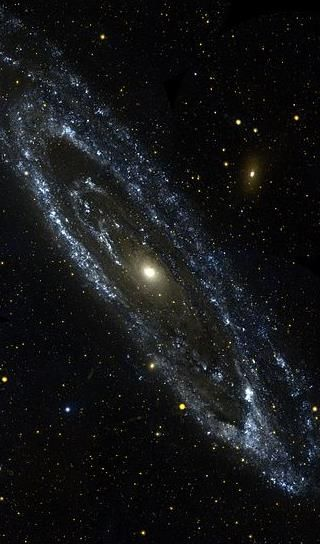
\includegraphics[width=\textwidth]{universe1}
	\end{subfigure}
	\begin{subfigure}[t]{0.45\textwidth}
		\caption{According to us}
		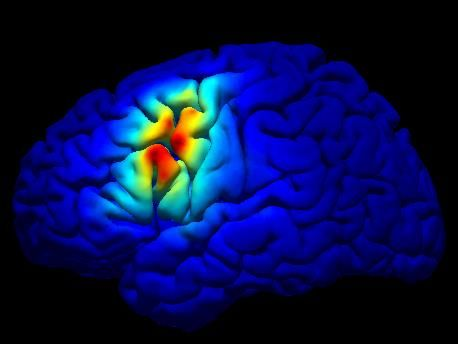
\includegraphics[width=\textwidth]{universe2}
	\end{subfigure}
\end{figure}
\subsubsection{Understanding the Brain using Computational Models}
\begin{itemize}
	\item Descriptive Models of the Brain
	\begin{itemize}
		\item How do neurons respond to external stimuli and how do we
		describe this quantitatively with a neural encoding model?
		\item How can we extract information from neurons (decoding)?
	\end{itemize}
    \item Mechanistic Models of Brain Cells and Networks
	\begin{itemize}
		\item     How can we simulate the behavior of a single neuron on a
	    computer?
	    \item How do we simulate a network of neurons?
	\end{itemize}
	\item  Interpretive (or Normative) Models of the Brain
	\begin{itemize}
		\item 	Why do brain circuits operate the way they do?
		\item What are the computational principles underlying their
		operation?
	\end{itemize}
\end{itemize}

\subsubsection{Course Goals: What you can expect to learn}
At the end of the course, you will be able to:
\begin{itemize}
	\item  Quantitatively describe what a biological neuron or
network of neurons is doing given experimental data
 \item Simulate on a computer the behavior of neurons and
networks
 \item Formulate computational principles underlying the
operation of neurons and networks in the brain
\end{itemize}

\subsection{Computational Neuroscience - Descriptive Models}

\subsubsection{Receptive Fields}
\begin{figure}[H]
	\caption[Responses of a Neuron in an Intact Cat Brain]{Responses of a Neuron in an Intact Cat Brain\cite{hubel1965receptive}}
	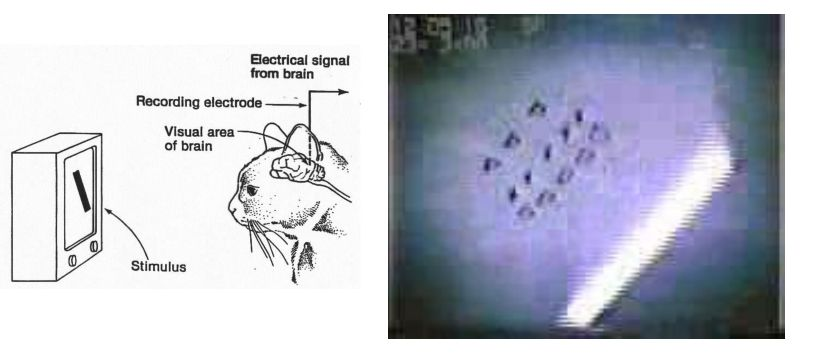
\includegraphics[width=\textwidth]{receptive-field-cat}
\end{figure}

\begin{figure}[H]
	\caption{Responses showing \gls{gls:rf}}
	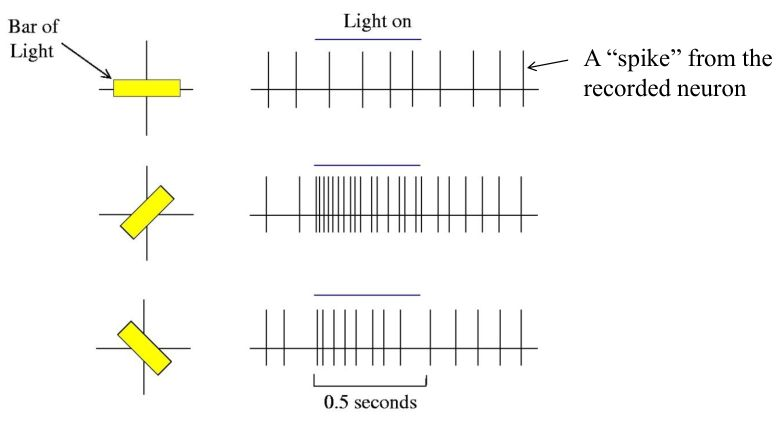
\includegraphics[width=\textwidth]{receptive-field-cat-bars}
\end{figure}

\subsubsection{Receptive Fields: a Descriptive Model}

\begin{figure}[H]
	\caption{Receptive Fields in the Retina}
	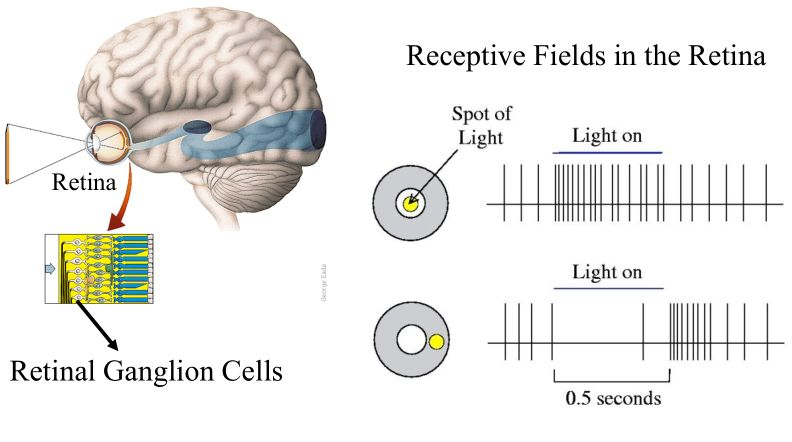
\includegraphics[width=0.8\textwidth]{receptive-fields-in-the-retina}
\end{figure}

\begin{figure}[H]
	\caption{Centre Surround Receptive Fields}
	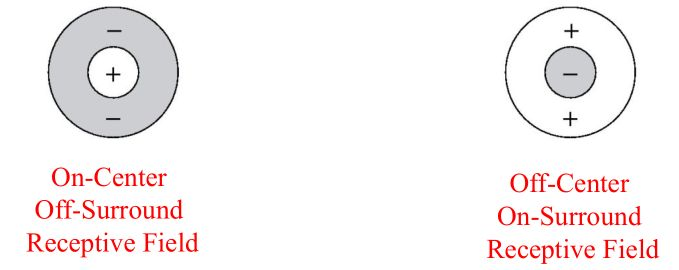
\includegraphics[width=0.8\textwidth]{center-surround}
\end{figure}

\begin{figure}[H]
	\caption{Cortical Receptive Fields}
	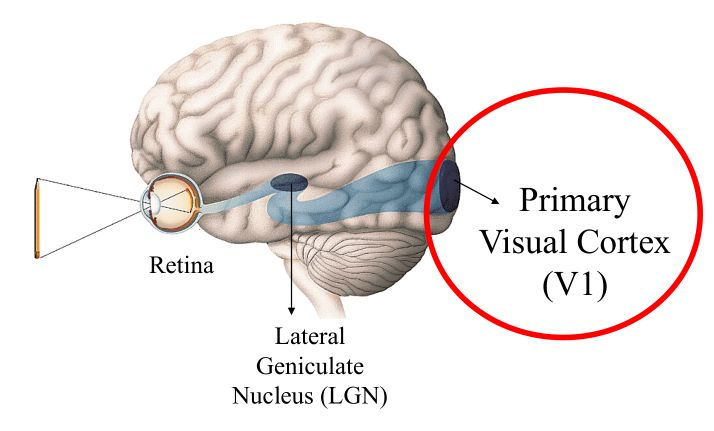
\includegraphics[width=\textwidth]{CorticalReceptive Fields}
\end{figure}

\begin{figure}[H]
	\caption{Oriented receptive field of a neuron in primary visual cortex (V1)}
	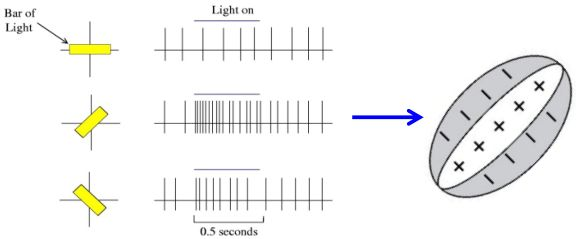
\includegraphics[width=\textwidth]{orientation-preference}
\end{figure}

\begin{figure}[H]
	\caption[How are these oriented receptive fields obtained?]{How are these oriented receptive fields obtained from center-surround receptive fields?}\label{fig:rf-shape}
	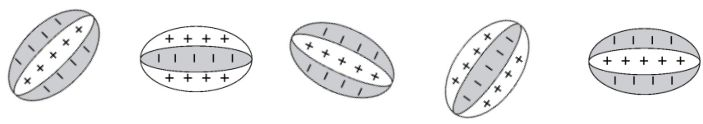
\includegraphics[width=\textwidth]{orientation-preference2}
\end{figure}

\subsection{Computational Neuroscience Mechanistic and Interpretive Models}


\begin{figure}[H]
	\caption[Receptive Fields: a Mechanistic Model]{Receptive Fields: a Mechanistic Model}
	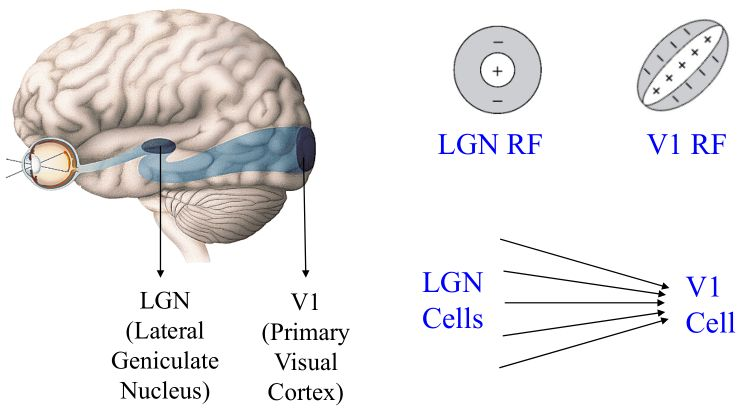
\includegraphics[width=0.9\textwidth]{mech-rf}
\end{figure}

\begin{figure}[H]
	\caption[Model suggested by Hubel \& Wiesel in the 	1960s]{Model suggested by 	Hubel \& Wiesel in the 	1960s: V1 RFs are 	created from converging
		LGN inputs. Center-surround LGN RFs are displaced along
		preferred orientation of V1 cell This simple model is still controversial!}
	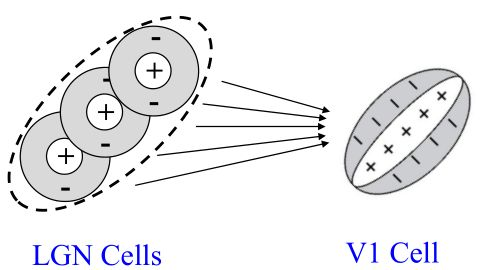
\includegraphics[width=0.9\textwidth]{mech-rf-v1}
\end{figure}

\subsubsection{Receptive Fields: an Interpretive Model}
Why are receptive fields in V1 shaped as in Figure \ref{fig:rf-shape}?

\begin{figure}[H]
	\caption[Efficient Coding Hypothesis]{Efficient Coding Hypothesis: suppose the
		goal is to represent images as faithfully and efficiently as possible using neurons with receptive fields $RF_1, RF_2$, etc}
	\begin{subfigure}[t]{0.2\textwidth}
		\caption{$RF_1$}
		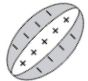
\includegraphics[width=0.7\textwidth]{rf1}
	\end{subfigure}
	\begin{subfigure}[t]{0.2\textwidth}
		\caption{$RF_2$}
		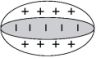
\includegraphics[width=\textwidth]{rf2}
	\end{subfigure}
	\begin{subfigure}[t]{0.2\textwidth}
		\caption{$RF_3$}
		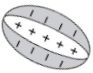
\includegraphics[width=\textwidth]{rf3}
	\end{subfigure}
	\begin{subfigure}[t]{0.2\textwidth}
		\caption{$RF_4$}
		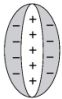
\includegraphics[width=0.5\textwidth]{rf4}
	\end{subfigure}
\end{figure}

Given image $I$, we can reconstruct it using neural responses $\{r_i\}$.
\begin{align*}
	\hat{I} =& \sum RF_i r_i
\end{align*}

What are the $RF_i$ that minimize the total squared pixelwise errors between $I$ and $\hat{I}$ and are as independent as possible?

\begin{figure}[H]
	\begin{center}
		\caption[Interpretive Model of Receptive Fields]{Interpretive Model of Receptive Fields: start out with random $RF_i$ and run your efficient coding algorithm on natural image patches}
		\begin{subfigure}[t]{0.9\textwidth}
			\begin{center}
				\caption{Natural Images}
				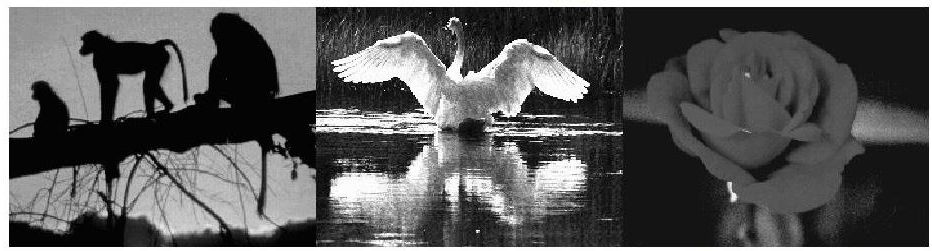
\includegraphics[width=0.7\textwidth]{natural-image}
			\end{center}
		\end{subfigure}
		\begin{subfigure}[t]{\textwidth}
			\caption{Receptive Fields from Natural Images}
			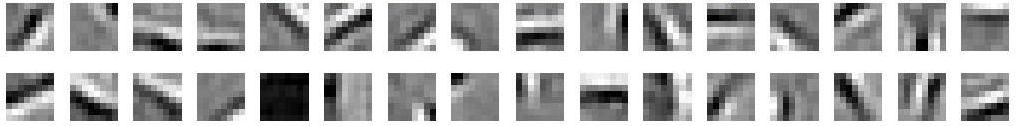
\includegraphics[width=\textwidth]{rf-natural}
		\end{subfigure}
		\begin{subfigure}[t]{\textwidth}
			\caption{Receptive Fields from V1, after Figure \ref{fig:rf-shape}}
			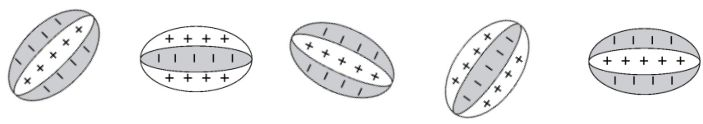
\includegraphics[width=\textwidth]{orientation-preference2}
		\end{subfigure}
	\end{center}
\end{figure}

 The brain may be trying to find faithful and efficient representations of an animal’s natural environment\cite{olshausen1997sparse,bell1997independent,rao1999predictive}

\subsection{The Electrical Personality of Neurons}

Originally there were two competing hypothesis:
\begin{itemize}
	\item the reticular hypothesis supposed that the brain was a continuous network;
	\item the \emph{neuron doctrine}:
	\begin{itemize}
		\item the neuron is the fundamental structural \& functional unit of the brain;
		\item neurons are discrete cells and not continuous with other cells;
		\item information flows from the dendrites to the axon via the cell body.
	\end{itemize}
\end{itemize}

\begin{figure}[H]
	\caption[The idealized Neuron]{The idealized Neuron. The \gls{gls:EPSP}s are summed: if the sum reaches a threshold, we get an action potential, also known as a spike.}
	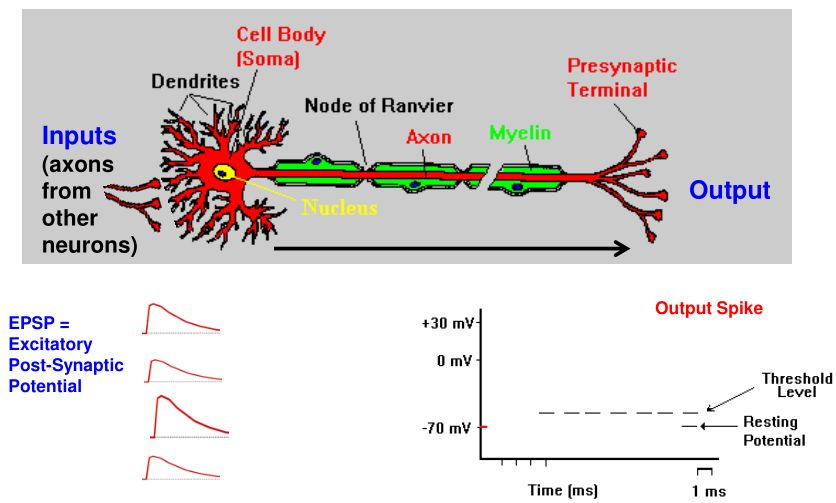
\includegraphics[width=0.9\textwidth]{idealized-neuron}
\end{figure}

\begin{figure}[H]
	\caption[What is a Neuron?]{What is a Neuron?}
	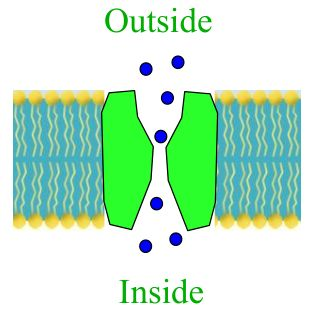
\includegraphics[width=0.9\textwidth]{what-is-a-neuron}
\end{figure}

\begin{itemize}
	\item  A ``leaky bag of charged liquid''
	\item Contents of the neuron enclosed within a cell membrane
	\item Cell membrane is a lipid bilayer
	\begin{itemize}
		\item Bilayer is impermeable to charged ion species such as $Na^+$ , $Cl^-$, and $K^+$
		\item Ionic channels embedded in 	membrane allow ions to flow in or out
	\end{itemize}
\end{itemize}

\begin{figure}[H]
	\caption[The Electrical Personality of a Neuron]{The Electrical Personality of a Neuron}
	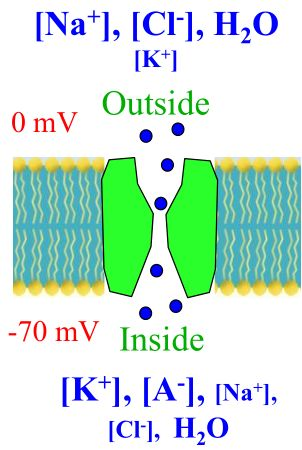
\includegraphics[width=0.9\textwidth]{what-is-a-neuron2}
\end{figure}

\begin{itemize}
	\item Each neuron maintains a potential difference across its membrane;
	\item Inside is about –70 mV relative to outside;
	\begin{itemize}
		\item sodium and chloride higher outside
		\item potassium and organic anions [$A^-$] higher inside
	\end{itemize}
	\item Ionic pump maintains -70 mV difference by expelling [$Na^+$] 
	and allowing [$K^+$] ions in. A lot of the energy that we consume is used to operate ionic pump.
\end{itemize}

How can the electrical potential be changed in local regions of a neuron?

\begin{figure}[H]
	\caption[Ionic Channels: the Gate Keepers]{Ionic Channels: the Gate Keepers.  Ionic channels  are selective and 	allow only specific ions to pass through}\label{fig:ionic-channel}
	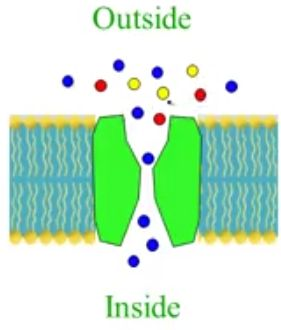
\includegraphics[width=0.9\textwidth]{ionic-channel}
\end{figure}

\begin{itemize}
	\item Ionic channels in membranes are proteins that are selective and allow only specific ions to pass through--Figure \ref{fig:ionic-channel}
	\item E.g. Pass $Na^+$ but not $K^+$ or $Cl^-$.
	\item Ionic channels are gated
	\begin{itemize}
		\item 	Voltage-gated: Probability of opening depends on membrane voltage
		\item Chemically-gated: Binding to a chemical causes channel to open--Figure \ref{fig:signalling}
		\item Mechanically-gated: Sensitive to 	pressure or stretch
	\end{itemize}
\end{itemize}

\begin{figure}[H]
	\caption[Gated Channels allow Neuronal Signaling]{Gated Channels allow Neuronal Signaling. The junctions between neurons are known as ``synapses''}\label{fig:signalling}
	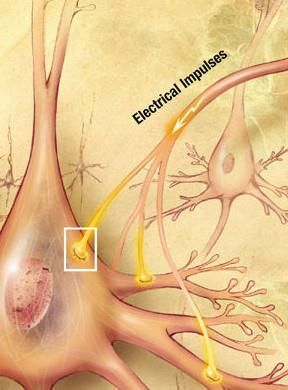
\includegraphics[width=0.9\textwidth]{signalling}
\end{figure}

\begin{itemize}
	\item Inputs from other neurons $\rightarrow$ 	chemically-gated channels (at
	``synapse'') open  $\rightarrow$ Changes in local membrane potential
	\item This in turn causes opening/closing 	of voltage-gated channels in 	dendrites, body, and axon, resulting in \gls{gls:depolarization} (\glsdesc{gls:depolarization}) or \gls{gls:hyperpolarization}	(\glsdesc{gls:hyperpolarization})
	\item Strong enough \gls{gls:depolarization}	causes a spike or “action potential”
\end{itemize}

\begin{figure}[H]
	\caption[The Output of a Neuron: Action Potential (Spike)]{The Output of a Neuron: Action Potential (Spike). Voltage-gated channels cause action potentials (spikes) Strong \gls{gls:depolarization} opens $Na^+$ channels, causing rapid $Na^+$ influx and more channels to open, until they inactivate; $K^+$ outflux restores membrane potential. The shape of the action potential is stereotypical, so no information is propagated by the shape.}
	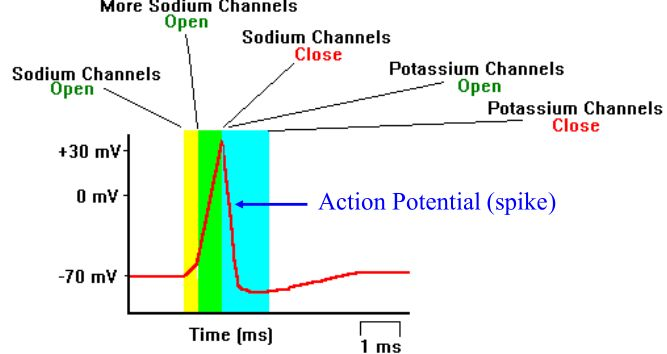
\includegraphics[width=0.7\textwidth]{action-potential}
\end{figure}

\begin{figure}[H]
	\caption[Propagation of a Spike along an Axon]{Propagation of a Spike along an Axon. At each point, the $Na^+$ rushes in first, followed by the $K^+$ rushing out\cite{krantz2000PsychScholar}}
	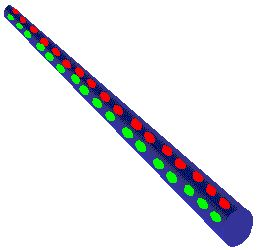
\includegraphics[width=0.7\textwidth]{propagation1}
\end{figure}



\begin{figure}[H]
	\caption[Active Wiring: Myelination of Axons]{Active Wiring: Myelination of Axons. Myelin due to oligodendrocytes (glial cells) wrap axons and
		enable fast long-range spike communication
		Action potential “hops” from one non-myelinated region
		(node of Ranvier) to the next (saltatory conduction)
		“Active wire” allows lossless signal propagation}
	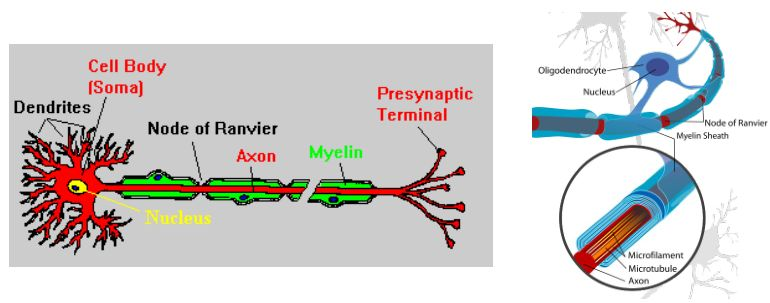
\includegraphics[width=0.9\textwidth]{myelination}
\end{figure}



\subsection{Making Connections - Synapses}
\begin{figure}[H]
	\caption[Enter the Synapse]{What happens to the spike (action potential) when	it reaches the 	end of an axon?	Enter the Synapse}\label{fig:enter:the:synapse}
	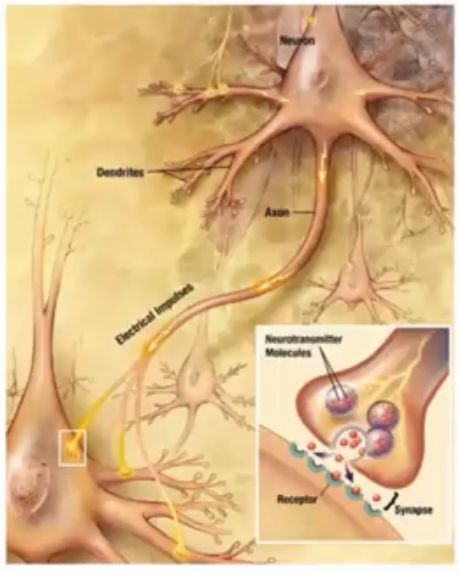
\includegraphics[width=0.9\textwidth]{enter-synapse}
\end{figure}

\begin{figure}[H]
	\caption[What is a Synapse?]{What is a Synapse?  a connection or junction between two neurons: Electrical synapses use gap junctions;	Chemical synapses use neurotransmitters.}
	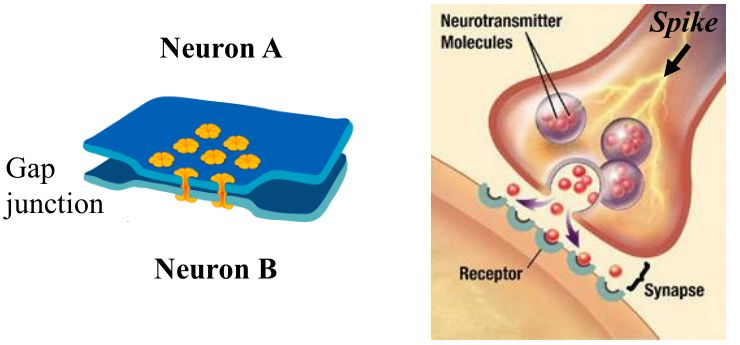
\includegraphics[width=0.9\textwidth]{synapse1}
\end{figure}

Why two mechanisms? Why would we evolve slow chemical synapses in addition to fast electrical ones? One possible answer is that we can adjust strength of coupling by changing the number of vesicles; it has been suggested that chemical synapses are the basis for learning and memory.
\begin{figure}[H]
	\caption[Distribution of synapses on a real neuron]{Distribution of synapses on a real neuron}
	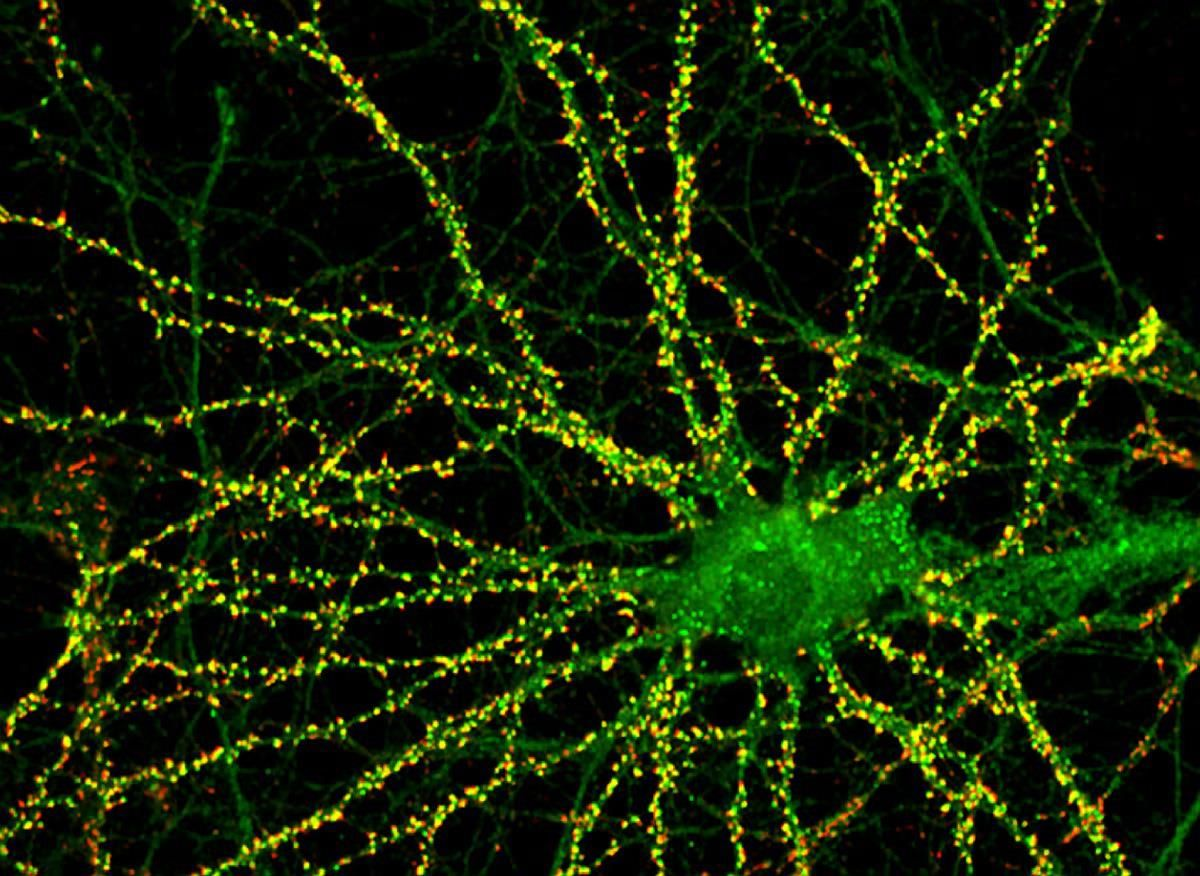
\includegraphics[width=0.9\textwidth]{synapse2}
\end{figure}

\begin{figure}[H]
	\caption[Synapses can be Excitatory or Inhibitory]{Synapses can be Excitatory or Inhibitory: increase or decrease postsynaptic membrane potential}
	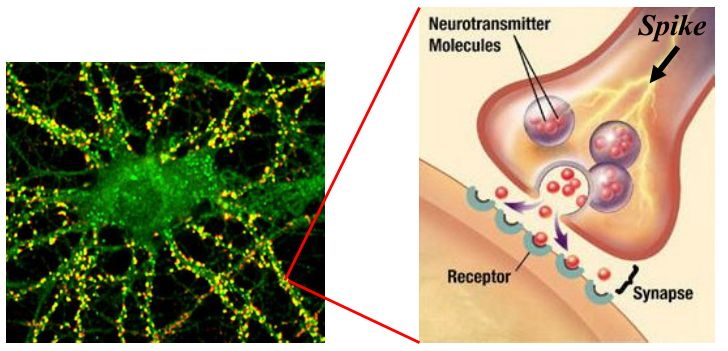
\includegraphics[width=0.9\textwidth]{synapse3}
\end{figure}

\begin{figure}[H]
	\caption[An Excitatory Synapse]{An Excitatory Synapse. Input spike  $\rightarrow$
		Neurotransmitter 	release (e.g., Glutamate)  $\rightarrow$ Binds to ion channel receptors $\rightarrow$ Ion channels open $\rightarrow$ $Na^+$ influx  $\rightarrow$ 	\Gls{gls:depolarization} due to \gls{gls:EPSP}}
	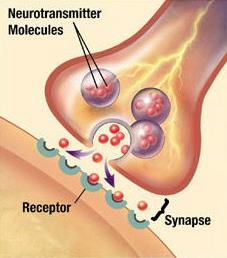
\includegraphics[width=0.9\textwidth]{synapse4}
\end{figure}

\begin{itemize}
	\item The Synapse Doctrine: Synapses are the basis for memory and learning
	\item Hebbian Plasticity--Figure \ref{fig:hebbian-plasticity}
	\item \acrfull{gls:LTP}:  \glsdesc{gls:ltp}
	\item \acrfull{gls:LTD}:  \glsdesc{gls:ltd}
\end{itemize}

\glsdesc{gls:ltd}

\begin{figure}[H]
	\caption[Hebbian Plasticity]{Hebbian Plasticity: if neuron A repeatedly takes part in firing neuron B, then the synapse from A to B is strengthened; neurons that fire together wire together!.}\label{fig:hebbian-plasticity}
	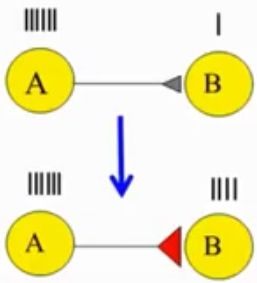
\includegraphics[width=0.9\textwidth]{hebbian-plasticity}
\end{figure}

\begin{figure}[H]
	\caption[Synaptic Plasticity depends on Spike Timing]{Synaptic Plasticity depends on Spike Timing. LTP/LTD depends on relative timing of input \& output spikes.}
	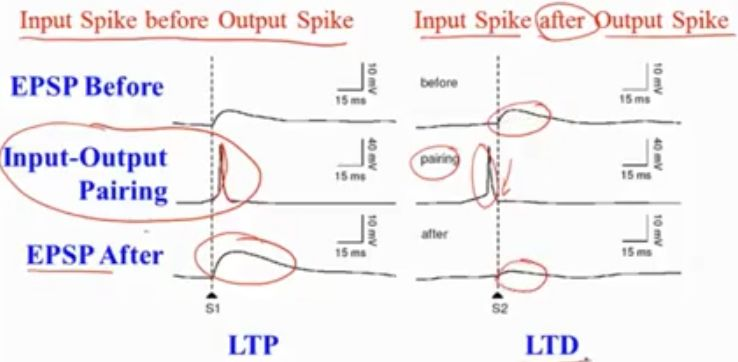
\includegraphics[width=0.9\textwidth]{ltp-ltd}
\end{figure}

\begin{figure}[H]
	\caption[\acrfull{gls:STDP}]{\acrfull{gls:STDP})\cite{bi2001synaptic}}
	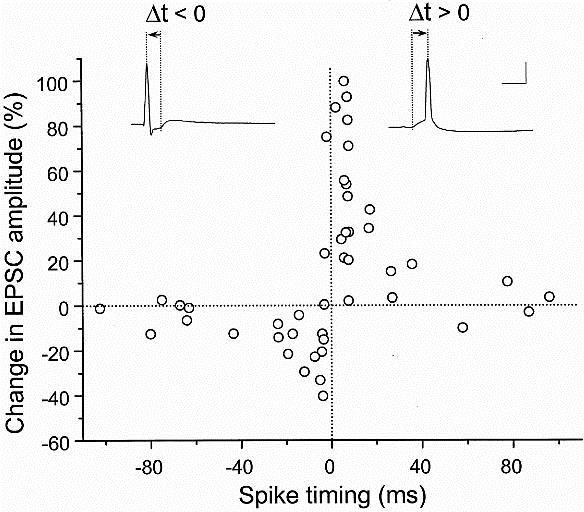
\includegraphics[width=0.9\textwidth]{stdp}
\end{figure}



\subsection{Time to Network - Brain Areas and their Function}

\begin{figure}[H]
	\caption{Brain Regions}
	\begin{subfigure}[b]{0.45\textwidth}
		\caption{Hind Brain. \emph{Medulla Oblongata} controls breathing, muscle tone and blood pressure.
			\emph{Pons} connected to the cerebellum \& involved in sleep and arousal.
			\emph{Cerebellum} Coordination and timing of voluntary movements, sense of equilibrium, language, attention}
		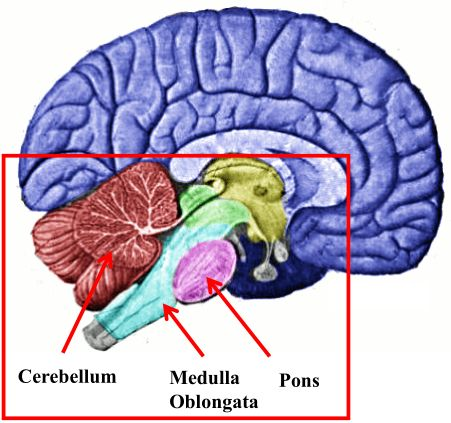
\includegraphics[width=\textwidth]{hindbrain}
	\end{subfigure}
	\begin{subfigure}[b]{0.45\textwidth}
		\caption{\emph{Midbrain} Eye movements, visual and auditory reflexes.
			\emph{Reticular Formation} 	Modulates muscle reflexes, breathing \& pain perception. Also regulates sleep, 			wakefulness \& 	arousal.}
		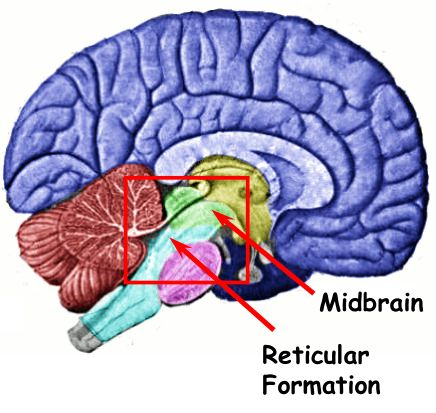
\includegraphics[width=\textwidth]{midbrain}
	\end{subfigure}
	\begin{subfigure}[b]{0.45\textwidth}
		\caption{\emph{Thalamus} Relay station for all 	sensory info (except 	smell) to the cortex, regulates sleep/wakefulness.
		\emph{Hypothalamus} Regulates basic needs: 	Fighting, Fleeing, 	Feeding, and Mating.}
		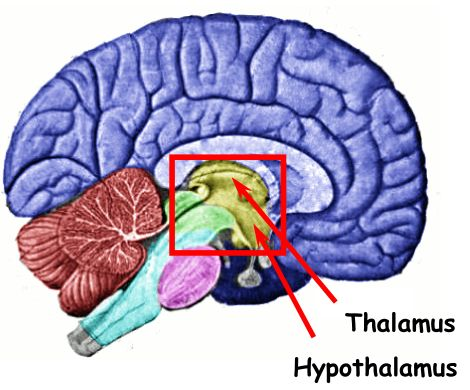
\includegraphics[width=\textwidth]{thalamus}
	\end{subfigure}
	\begin{subfigure}[b]{0.45\textwidth}
		\caption{ Consists of: Cerebral cortex, basal ganglia, 	hippocampus, and amygdala
		Involved in perception 	and motor control, 	cognitive functions,	emotion, memory, and learning}
		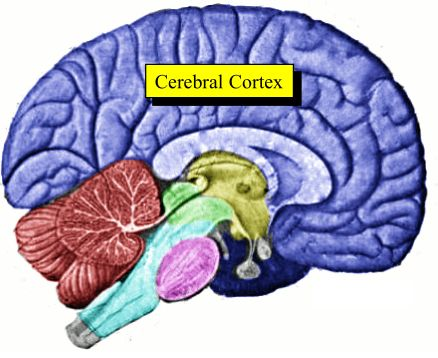
\includegraphics[width=\textwidth]{Cerebrum}
	\end{subfigure}
\end{figure}

\section{What do Neurons Encode?}\label{sec:week2}

\subsection{What is the Neural Code}
During this course, we will talk about:

\begin{itemize}
	\item techniques for recording from the brain--Figure \ref{fig:recording};
	\item  tools for discovering how the brain represents information;
	\item models that express our understanding of this representation;
	\item  some methods for inferring what the brain is doing based on its activity--Section \ref{sec:week3};
	\item  using information theory to quantify neural representations--Section \ref{sec:week4};
	\item the biophysical basis of how the brain processes inputs and performs complex computations--Section \ref{sec:week5}.
\end{itemize}

\begin{figure}[H]
	\caption[Recording from the Brain]{Recording from the Brain. (\subref{fig:rb1}) \& (\subref{fig:rb2}) \gls{gls:fMRI}: resolution $1\;mm^3$; response is averaged over many neurons, and is slow. (\subref{fig:rb3}) \gls{gls:EEG}: response is averaged over many neurons; EEG is faster than fMRI, but noisy. (\subref{fig:rb4}) \& (\subref{fig:rb5}) Electrode Arrays: good if we have access to tissue directly} \label{fig:recording} (\subref{fig:rb6} Calcium Imaging. Cells have markers that change the colour of fluorescence as calcium levels change in response to neural activity.)
	\begin{subfigure}[b]{0.3\textwidth}
		\caption{}\label{fig:rb1}
		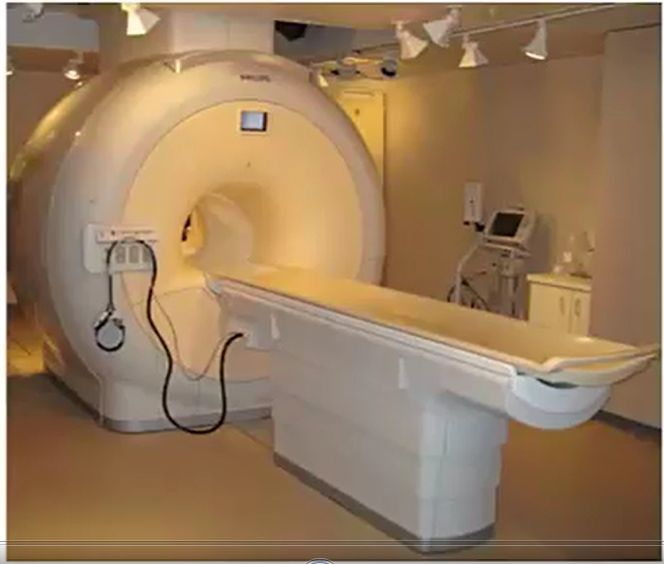
\includegraphics[width=0.9\textwidth]{fMRI}
	\end{subfigure}
	\begin{subfigure}[b]{0.3\textwidth}
		\caption{}\label{fig:rb2}
		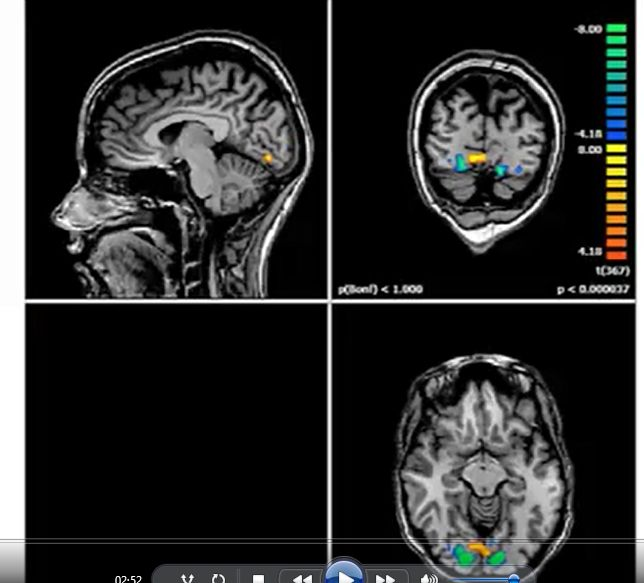
\includegraphics[width=0.9\textwidth]{fMRI2}
	\end{subfigure}
	\begin{subfigure}[b]{0.3\textwidth}
		\caption{}\label{fig:rb3}
		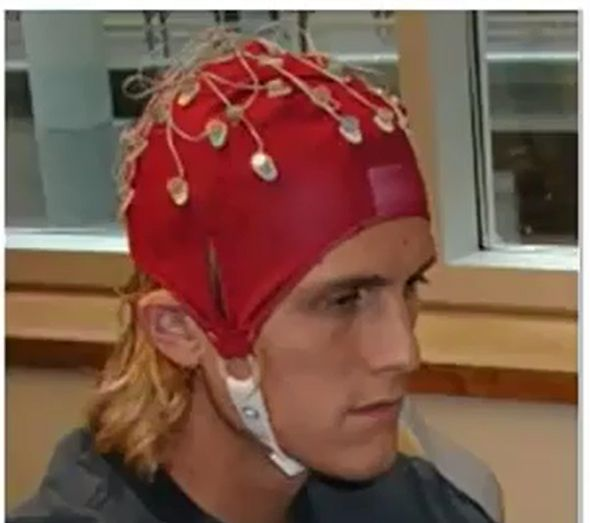
\includegraphics[width=0.9\textwidth]{EEG}
	\end{subfigure}
	\begin{subfigure}[b]{0.3\textwidth}
		\caption{}\label{fig:rb4}
		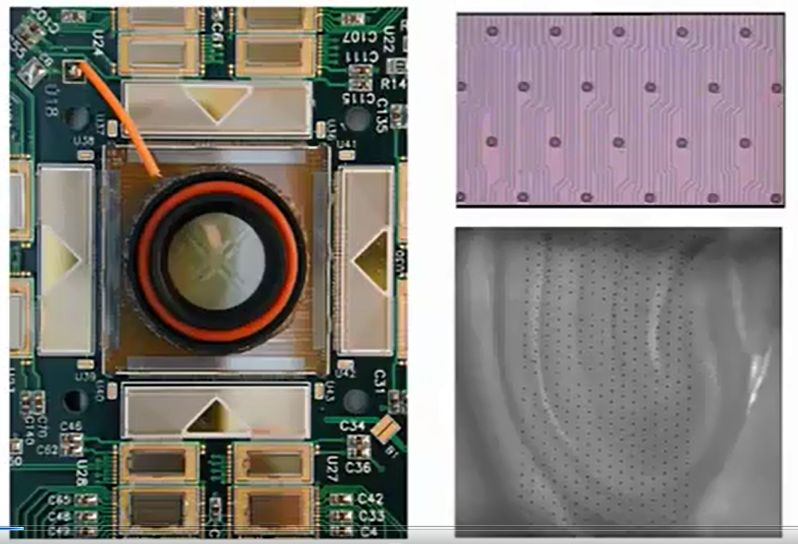
\includegraphics[width=0.9\textwidth]{electrode-arrays}
	\end{subfigure}
	\begin{subfigure}[b]{0.3\textwidth}
		\caption{}\label{fig:rb5}
		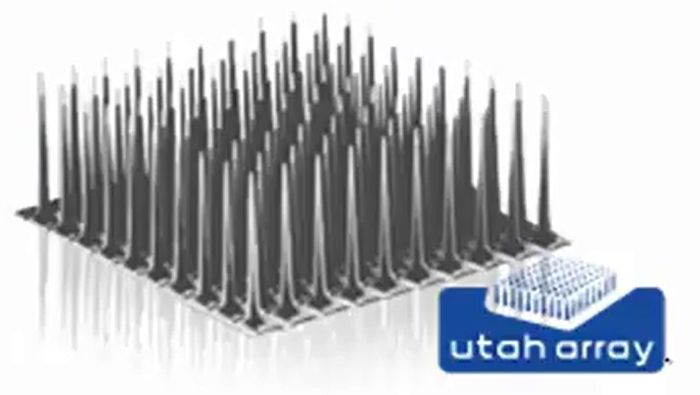
\includegraphics[width=0.9\textwidth]{electrode-arrays2}
	\end{subfigure}
	\begin{subfigure}[b]{\textwidth}
		\caption{}\label{fig:rb6}
		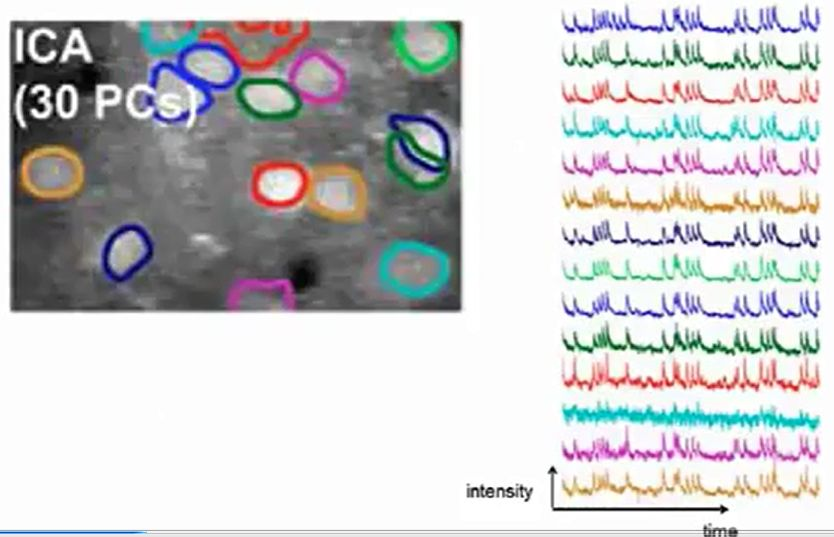
\includegraphics[width=0.9\textwidth]{calcium-imaging}
	\end{subfigure}
\end{figure}

\begin{figure}[H]
	\begin{center}
		\caption[Looking inside a single cell]{Looking inside a single cell. The experimenter clamps a patch electron onto the cell membrane}
		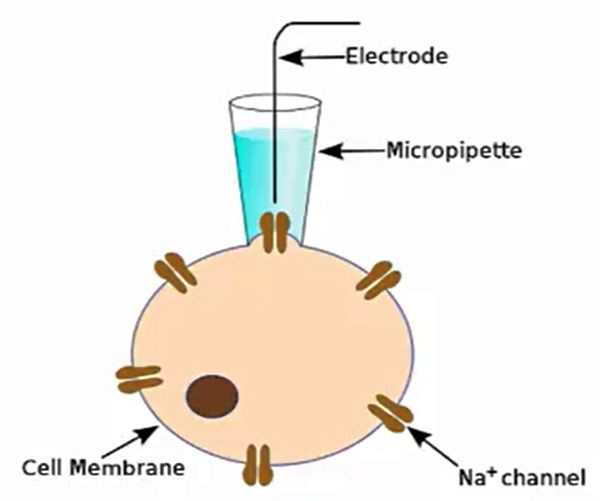
\includegraphics[width=0.9\textwidth]{looking-inside}
	\end{center}
\end{figure}

\begin{figure}[H]
	\begin{center}
		\caption{What is the neural code?}
		\begin{subfigure}[t]{0.45\textwidth}
			\caption{Human eye, without output to optic nerve}
			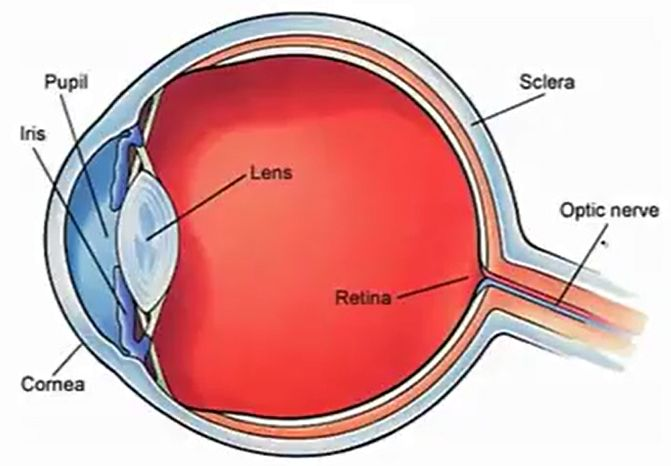
\includegraphics[width=\textwidth]{human-eye}
		\end{subfigure}
		\begin{subfigure}[to]{0.45\textwidth}
			\caption{Experiment. Play movie while section of retina is connected to electrode array--Figures \ref{fig:rb4} \& \ref{fig:rb5}}
			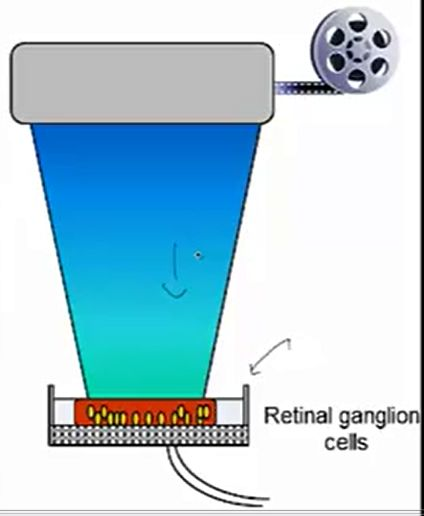
\includegraphics[width=\textwidth]{human-eye-experiment}
		\end{subfigure}
		\begin{subfigure}[to]{0.45\textwidth}
			\caption{Repeat experiment: red dots represent firings (action potentials). Notice that many times the firings are in almost the same place.}
			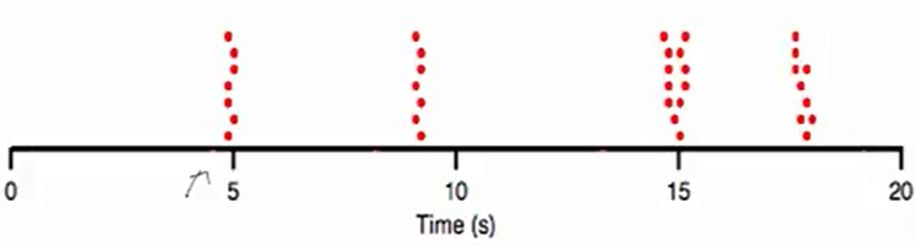
\includegraphics[width=\textwidth]{movie-firings}
		\end{subfigure}
		\begin{subfigure}[to]{0.45\textwidth}
			\caption{Look at 20 retinal ganglion cells. Each cell is reasonably consistent in time. Each cell is responsible for encoding some set of features, and different neurons encode different features. R \& P have some features in common.}\label{fig:movie-firings-20}
			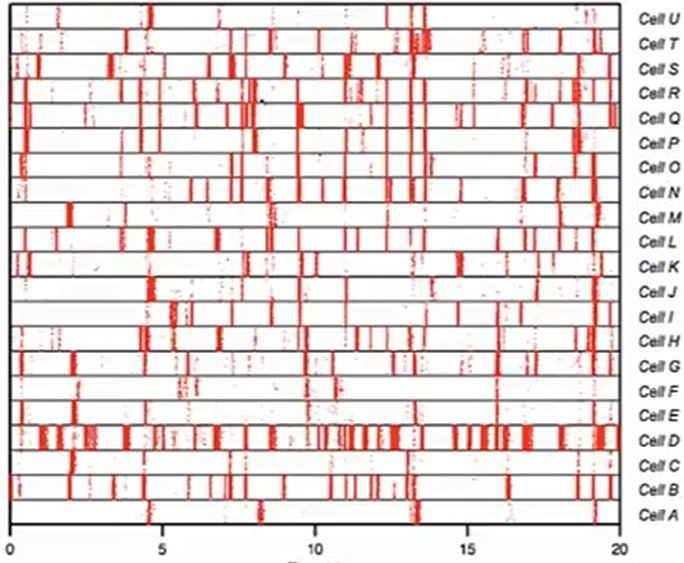
\includegraphics[width=\textwidth]{movie-firings-20}
		\end{subfigure}
	\end{center}
\end{figure}

\begin{itemize}
	\item Encoding: how does a stimulus cause a pattern of responses?
	\item\begin{itemize}
		\item  Building quasi mechanistic models
	\end{itemize}
	\item Decoding: what do these responses tell us about the stimulus?
	\item \begin{itemize}
		\item how can we reconstruct what the brain is doing?
	\end{itemize}
\end{itemize}

\begin{align*}
	P(response\vert stimulus)&\text{, encoding} \numberthis \label{eq:p_r_s}\\
	P(stimulus\vert response)&\text{, decoding}  \numberthis \label{eq:p_s_r}
\end{align*}

\begin{itemize}
	\item What is the stimulus--$s$?
	\item What is the response--$r$?
	\item what is the relation between them?
\end{itemize}
\begin{figure}[H]
	\begin{center}
		\caption[Gaussian tuning curve of a cortical (V1) neuron]{Gaussian tuning curve of a cortical (V1) neuron. These neurons respond to oriented bars.}
		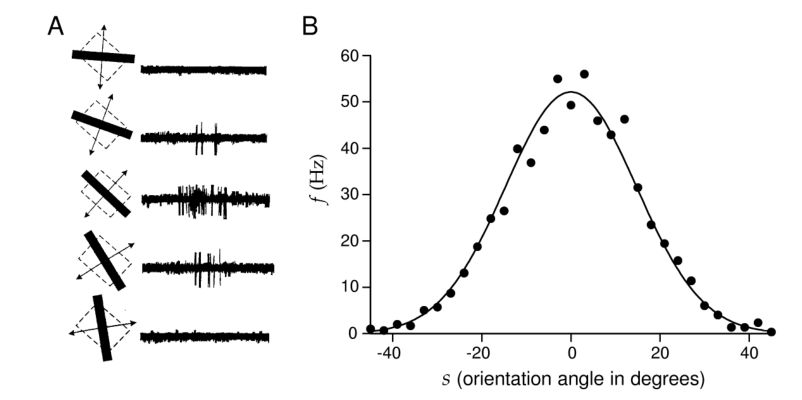
\includegraphics[width=0.9\textwidth]{tuning-curves}
	\end{center}
\end{figure}

\begin{figure}[H]
	\begin{center}
		\caption{Cosine tuning curve of a motor cortical neuron}
		\includegraphics[width=0.9\textwidth]{tuning-curves1}
	\end{center}
\end{figure}

\begin{figure}[H]
	\begin{center}
		\caption{Feature Map in Primary Visual Cortex}
		\includegraphics[width=0.9\textwidth]{feature-map}
	\end{center}
\end{figure}

\begin{figure}[H]
	\begin{center}
		\caption{Higher order features in temporal lobe}
		\includegraphics[width=0.9\textwidth]{higher-order-features}
	\end{center}
\end{figure}

\begin{figure}[H]
	\begin{center}
		\caption[Building up more complex features]{Building up more complex features. Notice feed-forward and feed-back.}
		\includegraphics[width=0.9\textwidth]{build}
	\end{center}
\end{figure}

\subsection{Neural Encoding - Simple Models}

We  consider the case where a response is a single spike. We want to determine $P(R\vert S) \rightarrow r(t)$, where $r(t)$ is the firing rate, given a stimulus $s$.

\begin{figure}[H]
	\begin{center}
		\caption{Simplest possible model: $r(t) = \phi s(t-\tau)$)}
		\includegraphics[width=0.9\textwidth]{simplest-model}
	\end{center}
\end{figure}

\subsubsection{What about a linear filter?}

\begin{align*}
	r(t) =& \sum_{i=1}^{n} s_{t-i} f_i \text{, or spatial filtering} \numberthis \label{eq:linear:filter}\\
	r(x,y) =& \sum_{x^\prime=-n,y^\prime=-n}^{n,n}s_{x-x^\prime,y-y^\prime} f_{x^\prime,y^\prime} \text{, as in Figure \ref{fig:rf1}}
\end{align*}

\begin{figure}[H]
	\begin{center}
		\caption[Receptive Field]{Receptive Field: (\subref{fig:rf1}) is a cartoon view, (\subref{fig:rf2}) shows the filter as a difference between two Gaussians; (\subref{fig:rf4}) shows the effect of applying the filter to (\subref{fig:rf3}.)}
		\begin{subfigure}[t]{0.45\textwidth}
			\caption{Cartoon}\label{fig:rf1}
			\includegraphics[width=0.9\textwidth]{receptive-field1}
		\end{subfigure}
		\begin{subfigure}[t]{0.45\textwidth}
			\caption{Detailed view}\label{fig:rf2}
			\includegraphics[width=0.9\textwidth]{receptive-field2}
		\end{subfigure}
		\begin{subfigure}[t]{0.45\textwidth}
			\caption{Taj Mahal}\label{fig:rf3}
			\includegraphics[width=0.9\textwidth]{receptive-field3}
		\end{subfigure}
		\begin{subfigure}[t]{0.45\textwidth}
			\caption{Filtered Taj Mahal, showing edges only}\label{fig:rf4}
			\includegraphics[width=0.9\textwidth]{receptive-field4}
		\end{subfigure}
	\end{center}
\end{figure}

\begin{figure}[H]
	\caption[Spatiotemporal filtering]{Spatiotemporal filtering. $r_{x,y}(t)=\int dx^\prime dy^\prime d\tau f(x^\prime,y^\prime,\tau) s((x-x^\prime,y-y^\prime,t-\tau)$}
	\includegraphics[width=0.9\textwidth]{spatio--temporal-filtering}
\end{figure}

\subsubsection{Linear filters cannot be the full picture}

Linear filters have a few limitations:
\begin{itemize}
	\item they can give rise to a negative firing rate!
	\item they can increase indefinitely!
\end{itemize} 

We need to impose a non-linearity, so \eqref{eq:linear:filter} becomes:
\begin{align*}
	r(t) =& g\big(\sum_{i=1}^{n} s_{t-i} f_i\big) \numberthis \label{eq:non-linearity}
\end{align*}

\begin{figure}[H]
	\caption{Filter showing effect of saturating non-linearity}
	\includegraphics[width=0.9\textwidth]{saturated}
\end{figure}

\subsection{Neural Encoding - Feature Selection}
How to find the components of \eqref{eq:non-linearity}? Our problem is dimensionality! We want to sample the responses of the system to many stimuli, so we can characterize what it is about the input that drives responses. We will start with a very high dimensional description and pick out a small set of relevant dimensions.

\begin{figure}[H]
	\caption[Dimensionality Reduction]{Dimensionality Reduction: $P(response|stimulus)\rightarrow P(response\vert s_1,s_2,...s_n)$}
	\includegraphics[width=0.9\textwidth]{dimenionality-reduction}
\end{figure}

Gaussian white noise is a useful method.

\begin{figure}[H]
	\caption[Determining multiple features from white noise]{Determining multiple features from white noise. This allows us to create a Gaussian prior. This will be a multivariate Gaussian, no matter which axes we use.}\label{fig:determining-multiple-features}
	\includegraphics[width=0.9\textwidth]{white-noise}
\end{figure}

\begin{figure}[H]
	\caption[Spike Conditioned Distribution]{Spike Conditioned Distribution. We project onto a vector representing mean of spike-conditioned points}\label{fig:spike:conditioned}
	\includegraphics[width=0.9\textwidth]{spike-conditioned-distribution}
\end{figure}

\begin{figure}[H]
	\caption[Reverse Correlation: the spike triggered average]{Reverse Correlation: the spike triggered average. Every time there is a spike, grab the portion of signal that preceded it, forming an ensemble, which we average. This represents what is common to stimuli that triggered response.}
	\includegraphics[width=0.9\textwidth]{reverse-correlation}
\end{figure}

\begin{figure}[H]
	\caption[Spike Triggered average for vector]{Spike Triggered average for vector, maybe in image that has been turned into a single vector}
	\includegraphics[width=0.9\textwidth]{sta-image}
\end{figure}

In each of these cases we have a vector that represents a feature, and we project the stimulus onto this unit vector. How do we compute the input-output curve, the function $g$ from \eqref{eq:non-linearity}? 

\begin{align*}
	P(spike\vert stimulus) \rightarrow& P(spike\vert s_1) \text{. This can be found using Bayes' rule.}\\
	 P(spike\vert s_1) =& \frac{\overbrace{P(s_1\vert spike)}^\text{Factor from Figure \ref{fig:factors:bayes}} \cdot \overbrace{P(spike)}^\text{Prior from Figure \ref{fig:determining-multiple-features}}}{\underbrace{P(s_1)}_\text{Factor from Figure \ref{fig:factors:bayes}}}
\end{align*}


\begin{figure}[H]
	\caption[Factors used in Bayes Rule]{Factors used in Bayes Rule}\label{fig:factors:bayes}
	\includegraphics[width=0.9\textwidth]{compondents-of bayes}
\end{figure}


\begin{figure}[H]
	\caption[Examples of IO curves]{Examples of IO curves. The left hand curve shows no impact from the stimulus; either there is none, or we have chosen the wrong vector.}\label{fig:sample-io-curves}
	\includegraphics[width=0.9\textwidth]{sample-io-curves}
\end{figure}

\subsubsection{High-dimensional Feature Selection}

We select some subset of features that are relevant to a decision: $r(t)=g(f_1*s, f_2*x,...)$. How can we extract more information from Figure \ref{fig:spike:conditioned}?

\begin{figure}[H]
	\caption[High-dimensional Feature Selection]{High-dimensional Feature Selection. We could extract higher order moments, or the covariance. Can use PCA to reduce dimensionality.}
	\includegraphics[width=0.9\textwidth]{spike-conditioned-distribution-covariance}
\end{figure}

\begin{figure}[H]
	\caption[Most faces can be reconstructed from a set of 7-8 eigenfaces]{Although it takes a lot of pixels to represent a face, there is a lot structure, and most faces can be reconstructed from a set of 7-8 principle components, known as ``eigenfaces''.}
	\includegraphics[width=0.9\textwidth]{eigenfaces}
\end{figure}

\begin{figure}[H]
	\caption[Use of PCA to sort out spikes]{Use of PCA to sort out spikes from two or more neurons recorded from a single electrode}
	\includegraphics[width=0.9\textwidth]{pca-spike-sorting}
\end{figure}

\begin{figure}[H]
	\caption[Finding Interesting Features in the Retina using PCA]{Finding Interesting Features in the Retina using PCA. Each blue dot represents 100 steps of a white-noise flicker. Spike triggered average is zero: we have two features, one which recognizes light turning on, the other off.}
	\includegraphics[width=0.9\textwidth]{finding-interestimg-features}
\end{figure}

\subsection{Neural Encoding - Variability}

There are a couple of things in Figure \ref{fig:movie-firings-20} that we still need to address: we modeled only a time varying firing rate, so thee are hidden assumptions about the rates at which signals and responses vary. There appears to be some fins structure that we have missed.

When have you found a good feature or features?
\begin{itemize}
	\item When the input/output curve over your variable is interesting
	\item How to quantify interesting?
\end{itemize}

\subsubsection{Quantifying Interesting}
In Figure \ref{fig:sample-io-curves}, the left hand curve is boring, the right interesting. Can we exploit the tuning curve and find a $f$ that maximizes the difference between the prior and posterior?

\begin{align*}
	P(spike\vert s_f) =&\frac{ P(s_f\vert spike) P_({spike})}{P(s_f)}
\end{align*}
 We introduce the Kullback-Leibler divergence
\begin{align*}
		D_{KL}(P(s),Q(s))\triangleq&\mathbb{E}_{P(s)} \Big(\log_2 \frac{P(s)}{Q(s)}\Big) \text{, and maximize}\\
		D_{KL}(P(s_f|spike),P(s_f))
\end{align*}

\begin{figure}[H]
	\caption[Maximally Informative Dimensions]{Maximally Informative Dimensions: choose filter to maximize $K_{DL}$ between spike-conditioned and prior distributions. This turns out to be equivalent to maximizing mutual information-\eqref{eq:mutual:information}. Notice that the stimulus is not necessarily Gaussian.}
	\includegraphics[width=0.9\textwidth]{maximally-informative-dimensions}
\end{figure}
This technique:
\begin{itemize}
	\item does not depend on white noise inputs;
	\item can be used for deriving models from natural stimuli;
	\item but is not guaranteed to give rise to a unique maximum.
\end{itemize}

Summary--finding relevant features:
\begin{enumerate}
	\item single filter determined by the conditional average;
	\item  a family of filters derived using PCA;
	\item information theoretic methods use the whole distribution.
\end{enumerate}

\subsubsection{Modelling the noise}

We can model spikes that may or may not occur with a series of time bins, each of which may or may not contain a spike. In the limit where there are many bons we can use the Poisson distribution.

\begin{align*}
	P_T(k) =& (rT)^k\frac{\exp(-rT)}{k!}\\
	<k> =& rT\\
	var(k) =& rT\\
	F =& 1 \text{, Fano factor}\\
	P(T)=&r \exp(-rT)
\end{align*}

\begin{figure}[H]
	\caption[Poisson or not?]{Poisson or not? Monkey is watching a movie. Rate is variable. Split time into bins and plot mean number of spikes and variance in each bin. Firing rate changes, but Fano remains close to 1.}
	\includegraphics[width=0.9\textwidth]{poisson-or-not}
\end{figure}

\begin{figure}[H]
	\caption[Interspike Interval Distributions]{Interspike Interval Distributions. A typical cortical neuron is connected to 10,000 others: average input may be zero, but there will be some jitter. Right hand image zooms in on short intervals, which are no longer Poisson for a good reason: a neuron's firing rate is limited by physics.}
	\includegraphics[width=0.9\textwidth]{interspike-intervals}
\end{figure}

\begin{figure}[H]
	\caption[Generalized Linear Model]{Generalized Linear Model\cite{pillow2008spatio}. $P(spike\;at\;t) \propto \exp(f_1*s + h_1*r)$. The exponential nonlinearity allows all parameters to be determined using an optimization scheme that is globally convergent.}
	\includegraphics[width=0.9\textwidth]{generalized-linear-model}
\end{figure}

\begin{figure}[H]
	\caption[Coupled Spiking Model]{Coupled Spiking Model\cite{pillow2008spatio}. $P(spike\;at\;t) \propto \exp(f_1*s + h_1*r_1+h_2*r_2)$.}
	\includegraphics[width=0.9\textwidth]{coupled-spiking-model}
\end{figure}

\begin{figure}[H]
	\caption[Time Rescaling Theorem]{The Time Rescaling Theorem\cite{brown2002time} allows us to determine whether we have captured everything we can from the inputs to out model. Scale output time intervals by firing rate that model predicted. If predicted rate accounts for all the influences on the firing, then scaled intervals should be distributed like a pure Poisson process with an effective rate of 1.} 
	\includegraphics[width=0.9\textwidth]{time-rescaling-thorem}
\end{figure}

\section{Extracting Information from Neurons}\label{sec:week3}

\subsection{Neural Decoding and Signal Detection Theory}
See \cite{britten1992analysis}
\begin{figure}[H]
		\caption[Value of threshold that maximizes probability of correct call]{This value of threshold maximizes probability of calling correctly.
			$p[+]p[r\ge z\vert +] + p[-] (1-p[r\ge z\vert -])$}
		\includegraphics[width=\textwidth]{signal-detection1}
\end{figure}
\subsection{Population Coding and Bayesian Estimating}

\begin{align*}
	\underbrace{p[s\vert r]}_\text{A posteriori distribution} =& \frac{\overbrace{p[r\vert s]}^\text{Likelihood function} \cdot \overbrace{p[s]}^\text{Prior distribution}}{\underbrace{p[r]}_\text{Marginal distribution}} \text{, where}\\
	p[r] =& \int ds \; p[r\vert s] p[s]
\end{align*}

\begin{itemize}
	\item \gls{gls:ML} \gls{gls:mlm}
	\item \gls{gls:MAP} \gls{gls:mpm}
\end{itemize}
 An example. Assume:
 
\begin{enumerate}
	\item a population of neurons that encode some stimulus $s$
	\item response is Gaussian (e.g. V1)
	\item each fires independently
	\item Poisson Firing\label{item:poisson}
\end{enumerate}

\begin{figure}[H]
	\caption{Gaussian Tuning Curves}
	\includegraphics[width=\textwidth]{decode-stimulus}
\end{figure}

\begin{align*}
	f_a(s) =& r_{max} \exp \Big(-\frac{1}{2}\big[\frac{s-s_a}{\sigma_a}\big]^2\Big)\text{, assume good coverage} \numberthis \label{eq:gauss}\\
	\sum_{1}^{N} f_a(s) =& const \numberthis \label{eq:good:coverage}
\end{align*}

So firing rate doesn't depend on stimulus

From assumption \ref{item:poisson}, spikes are produced randomly and independently in each time bin with probability
\begin{align*}
	P_T[k] =& \frac{(rT)^k \exp (-rT)}{k!}\\
	P_T[r_a\vert s] =& \frac{(f_a(s)T)^{r_aT} \exp (-f_a(s)T)}{r_aT!}\\
	P[\vec{r}\vert s] =& \prod_{a=1}^{N}P_r[a\vert s]\\
	=& \prod_{a=1}^{N} \frac{(f_a(s)T)^{r_aT} \exp (-f_a(s)T)}{r_aT!}
\end{align*}

We want the \gls{gls:ML} for $s$.
\begin{align*}
	\ln P[\vec{r}\vert s] =& \sum_{a=1}^{N} \big[r_aT \ln (f_a(s)T) -f_a(s)T - \ln (r_aT!) \big] \text{, so we need}\\
	\nabla_a \ln P[\vec{r}\vert s] =& 0	
\end{align*}
 where  $\nabla_a$ denotes the operator $\frac{\partial}{\partial_{s_a}}$. Now
\begin{align*}
	\nabla_a \ln P[\vec{r}\vert s] = & \partial_a \sum_{a=1}^{N}  r_aT \ln (f_a(s)T) -\underbrace{\partial_a \sum_{a=1}^{N} f_a(s)T}_{=0 \text { from ]\eqref{eq:good:coverage}}} - \underbrace{\partial_a \sum_{a=1}^{N} \ln (r_aT!)}_{=0} 
\end{align*}
Hence the \gls{gls:mlm} is given by:
\begin{align*}
	T \partial_a \sum_{a=1}^{N} r_a  \ln (f_a(s)T) =& 0\\
	 \sum_{a=1}^{N} r_a  \partial_a \ln (f_a(s)T) =& 0\\
	 \sum_{a=1}^{N} r_a  \frac{\partial_a  (f_a(s)\cancel{T})}{(f_a(s)\cancel{T})} =& 0\\
	 \sum_{a=1}^{N} r_a  \frac{\partial_a  f_a(s^*)}{f_a(s^*)} =& 0 \numberthis \label{eq:ml:example}
\end{align*}

\begin{align*}
	\partial_a  f_a(s) =& \partial_a r_{max} \exp \Big(-\frac{1}{2}\big[\frac{s-s_a}{\sigma_a}\big]^2\Big)\\
	=&r_{max}\big[-\frac{1}{\cancel{2}} \frac{\cancel{2}(s-s_a)}{\sigma_a^2}\big] \exp \Big(-\frac{1}{2}\big[\frac{s-s_a}{\sigma_a}\big]^2\Big)\\
	=& \frac{\cancel{2}(s-s_a)}{\sigma_a^2} f_a(s) \text{, so \eqref{eq:ml:example} becomes}
\end{align*}
\begin{align*}
	\sum_{a=1}^{N} r_a  \frac{(s^*-s_a)}{\sigma_a^2} =& 0\\
	s^*  =& \frac{\sum_{a=1}^{N}   \frac{s_a r_a}{\sigma_a^2}}{\sum_{a=1}^{N} \frac{ r_a }{\sigma_a^2}}	\\
	=& \frac{\sum_{a=1}^{N}   p_a s_a r_a}{\sum_{a=1}^{N} p_a r_a} \text{, where the precision $p_a=\sigma_a^{-2}$}\\
	=& \frac{\sum_{a=1}^{N}   s_a r_a}{\sum_{a=1}^{N} r_a} \text{, if all the $s_a$ are equal}
\end{align*}

For the \gls{gls:MAP} estimate, Bayes rule gives:
\begin{align*}
	\ln p[s|r] =& \ln p[r|s] + \ln p[s] - \ln p[r]\\
	=& T \sum_{a=1}^{N}r_a \ln f_a(s) + \ln p[s] + C \text{, where $C$ does not depend on $s_a$}
\end{align*}

So the \gls{gls:MAP} estimator satisfies:
\begin{align*}
	\sum_{a=1}^{N} r_a \frac{f^\prime(a^*)}{f(a^*)} + \frac{p^\prime(s)}{p(s)}=&0\\
	s^*  =& \frac{\sum_{a=1}^{N}   \frac{s_a r_a}{\sigma_a^2}+\frac{s_{prior}}{\sigma_{prior}^2}}{\sum_{a=1}^{N} \frac{ r_a }{\sigma_a^2}+\frac{1}{\sigma_{prior}^2}}
\end{align*}
\subsection{Reading Minds - Stimulus Reconstruction}
We want an estimator, $S_{Bayes}$ that gives the "best" estimate of $s$ given $r$.

\section{Entropy \& Spike Trains}\label{sec:week4}

\subsection{Information \& Entropy}

Entropy measures surprise.
\begin{align*}
	H =& - \sum_{i} p_i \log_2 p_i
\end{align*}

\begin{figure}[H]
	\begin{center}
		\caption{How about the stimulus?}
		\includegraphics[width=0.8\textwidth]{how}\label{fig:how:about:the:stimulus}
	\end{center}
\end{figure}

In Figure \ref{fig:how:about:the:stimulus}, suppose the probability of error is a constant.
\begin{align*}
	P[r_-\vert +] =& q\\
	P[r_+\vert +] =& 1-q\\
	P[r_+\vert -] =& q\\
	P[r_-\vert -] =& 1-q
\end{align*}
\begin{align*}
	H[R] =& -P[r_+] \log P[r_+] - P[r_-] \log P[r_-] \text{, total entropy}\\
	H[R\vert +] =& -q \log q - (1-q) \log (1-q) \text{, noise entropy}
\end{align*}


Mutual Information: total entropy - average noise entropy.

\begin{align*}
	I(R,S) =& -\sum_r p[r] \log p[r] - \sum_s p(s)\big[- \sum_r p[r \vert s] \log p[r \vert s]\big]\\
	=& H[R] - \sum_s p(s) H[R\vert s] \numberthis \label{eq:mutual:information}\\
\end{align*}
\begin{align*}
	I[S,R] \triangleq D_{KL}&\big[P(R,S),P(R)P(S)\big]\\
	=&H[R]-\sum_s P(s) H[R\vert s]
\end{align*}

\subsection{Calculating Information in Spike Trains}

What information is carried by patterns of spikes?

Mutual  information  is  the  difference  between  
the  total  response  entropy  and   the  mean  noise  entropy.
\begin{align*}
	I(S;R) =& H[R] - \sum_s P[s] H[R\vert s]
\end{align*}
\begin{figure}[H]
	\begin{center}
			\caption[Calculating Information in Spike Patterns]{Calculating Information in Spike Patterns. Divide into words of length $T$, e.g. $w_1=[1,0,1,0,1,1,0]$. Information is difference between total variability driven by stimuli and that dues to noise, averaged over stimuli.\cite{strong1998entropy}}
		\includegraphics[width=\textwidth]{calculatingInformationInSpikePatterns}
	\end{center}
\end{figure}

\begin{figure}[H]
	\begin{center}
		\caption[Entropy for chunked words]{Entropy for chunked words. The most common pattern is all zeroes, then a single bit, etc. nformation  :   
			difference  between  the  total  
			variability   driven  by  stimuli  
			and  that  due  to   noise,  averaged  
			over  stimuli. \cite{strong1998entropy,reinagel2000temporal}}
		\includegraphics[width=\textwidth]{info-spike-trains}
	\end{center}
\end{figure}
\subsection{Coding Principles}
\begin{itemize}
	\item What are the challenges posed by natural stimuli?
	\item What do information theoretic concepts suggest that neural systems should do?
	\item What principle seems to be at work shaping the neuarl code?
\end{itemize}

Photo - have to change F-stop repeatedly in order to capture details of scene inside and outside; the eye does this effortlessly. Natural stimuli:
\begin{enumerate}
	\item Have a wide dynamic range: variations over many orders of magnitude;
	\item dynamic scaling.
\end{enumerate}

\begin{figure}[H]
	\begin{center}
		\caption[Power Law]{Power Law: there are similar structures at very different length scales.}
		\begin{subfigure}[b]{0.45\textwidth}
			\caption{Structures}
			\includegraphics[width=0.9\textwidth]{power-law-graph}
		\end{subfigure}
		\begin{subfigure}[b]{0.45\textwidth}
			\caption{Power Spectrum: there is no characteristic scale for image.}
			\includegraphics[width=0.9\textwidth]{power-law-shapes}
		\end{subfigure}
	\end{center}
\end{figure}

\begin{figure}[H]
	\begin{center}
		\caption[Efficient Coding]{Efficient Coding: In order to have maximum entropy output, a good encoder should match its outputs to the distribution of its inputs. Try to use all symbols equally often. (cumulative probability)}
		\includegraphics[width=0.8\textwidth]{efficient-coding}
	\end{center}
\end{figure}

Contrast varies widely in time. Should neural system optimize locally or over evolutionary time?

\begin{figure}[H]
	\begin{center}
		\caption{What have we left out}
		\includegraphics[width=0.8\textwidth]{4-big-picture}
	\end{center}
\end{figure}

Make sure we have covered
\begin{enumerate}
	\item Efficient coding
	\item Sparse Coding
\end{enumerate}

\begin{align*}
	I(\vec{x}) =& \sum_{i}a_i \phi_i(\vec{x}) + \epsilon(\vec{x})\\
	E =& \mathlarger \sum_{\vec{x}}\big[I(\vec{x})-\sum_{i}a_i \phi_i(\vec{x})\big]^2 + \lambda \sum_{i}C(a_i)
\end{align*}


\section{Computing in Carbon}\label{sec:week5}

\subsection{Modeling Neurons}

\begin{figure}[H]
	\caption[Equivalent Circuit Model]{Equivalent Circuit Model: our goal is to develop a circuit diagram that models a neuron, using Kirchhoff's laws}
	\includegraphics[width=0.9\textwidth]{equivalent-circuit-model}
\end{figure}

\begin{figure}[H]
	\caption[Membrane Patch]{Membrane Patch}
	\includegraphics[width=0.9\textwidth]{membrane-patch}
\end{figure}

\begin{figure}[H]
	\caption[The passive membrane]{The passive membrane}
	\includegraphics[width=0.9\textwidth]{passive-membrane}
\end{figure}

\begin{align*}
	I_R + I_C + I_{ext} =& 0 \text{, Kirchhoff's Law}\\
	V =& I_R R \text{, Ohm's Law}\\
	I_C =& C \frac{dV}{dt} \text{, lipid bilayer asks as capacitor, plus allows a current to flow.}\\
	F\frac{dV}{dt} =& -\frac{V}{R} + I_{ext} \numberthis \label{eq:1st:neuron:eq}
\end{align*}

\begin{figure}[H]
	\caption[The Cell has a battery]{The Cell has a battery}
	\includegraphics[width=0.9\textwidth]{cell-has-battery}
\end{figure}

\begin{figure}[H]
	\caption[The cell's battery: the equilibrium potential]{The cell's battery: the equilibrium potential}
	\includegraphics[width=0.9\textwidth]{equilibrium-potential}
\end{figure}

Equilibrium is determined by the Nernst potential\cite{enwiki:1121504046}:
\begin{align*}
	E =& \frac{k_B T}{zq}\ln \frac{[inside]}{[outside]} \text{, where}\\
	k_B=& Boltzmann's constant\\
	T=& \text{ Temperature}\\
	q=& \text{ the ionic charge}\\
	z=&	\text{ the number of charges in the ion}
\end{align*}

Whence \eqref{eq:1st:neuron:eq} becomes
\begin{align*}
		C\frac{dV}{dt} =& -\frac{(-V-V_{rest})}{R} + I_{ext} \text{, or}\\
	\tau \frac{dV}{dt} =& -V + V_\infty \text{, where}\\
	\tau =& R C \text{, and} \\
	V_\infty =& \text{ represents the steady state}
\end{align*}

\begin{figure}[H]
	\caption[Example Solution]{Example Solution}
	\includegraphics[width=0.9\textwidth]{neuron-solution}
\end{figure}





\begin{figure}[H]
	\caption[Currents through Ion Channels]{Currents through Ion channels. }\label{eg:ion-channels}\label{fig:ion-channels}
	\includegraphics[width=0.9\textwidth]{ion-channels}
\end{figure}

Figure \ref{eg:ion-channels} depicts ion channels. There are different types: \begin{itemize}
	\item voltage dependent; 
	\item transmitter dependent (synaptic); 
	\item Ca dependent; 
	\item mechanosensitive;
	\item heat sensitive.
\end{itemize}
We will focus on voltage sensitivity, and will consider the current through one channel, $I=Vg$, where $g=\frac{1}{R}$ is the conductance of the channel. Different ion channels have different conductances; a given conductance tends to move the membrane potential towards the equilibrium potential for that ion.
\begin{table}[H]
	\begin{center}
		\caption[Examples of equilibrium potentials]{Examples of equilibrium potentials. Notice that sodium tends to depolarize, and potassium to polarize.}
		\begin{tabular}{|l|r|} \hline
			$E_{Na}$&50mV \\ \hline
			$E_{Ca}$&150mV \\ \hline
			$E_{K}$&-80mV \\ \hline
			$E_{Cl}$&-60mV \\ \hline
		\end{tabular}
	\end{center}
\end{table}

\begin{figure}[H]
	\caption[Current through ion channel]{Current through ion channel}
	\includegraphics[width=0.9\textwidth]{ion-channels3}
\end{figure}


\begin{figure}[H]
	\caption[What makes a neuron compute?]{What makes a neuron compute? So far everything we have seen is linear. But this figure shows that something else is happening...Excitability}
	\includegraphics[width=0.9\textwidth]{what-makes-neuron-compute}
\end{figure}


\subsection{Spikes}

\begin{figure}[H]
	\caption[Excitability arises from non-linearity]{Excitability arises from non-linearity. The equivalent circuit depicts the sodium and potassium currents, together with $g_L$, the \emph{leakage current} through the bilayer. If all conductances were constant we'd still have a linear response; the conductances depend on the voltage, however, which gives rise to non-linearity}
	\includegraphics[width=0.9\textwidth]{excitability-arises-from-non-linearity}
\end{figure}

\begin{figure}[H]
	\begin{center}
		\caption[The ion channel is an elaborate molecular machine]{The ion channel is an elaborate molecular machine. It contains a gate that prevents ions from entering, which is controlled by a sensor. The sensor for the potassium subchannel contains 4 subunits, so the probability of it being open is $P_k \propto n^4$ (The lower panel in Figure \ref{fig:ion-channels} depicts the flow when all 4 gates are open, vs the flow when at least one is closed). This probability increases when depolarized.}
	\includegraphics[width=0.6\textwidth]{ion-channel-as-molecular-machine}
	\end{center}
\end{figure}
State transitions occur at voltage dependent rates.
\begin{align*}
	\frac{dn}{dt} =& \alpha_n(V)(1-n) - \beta(V)n \numberthis \label{eq:n}\\
	\tau_n(V) \frac{dn}{dt} =&n_\infty(V)-n\text{, where}\\
	\tau_n(V) =& \frac{1}{\alpha_n(V) + \beta_n(V)}\\
	n_\infty(V) =&  \frac{\alpha_n(V)}{\alpha_n(V) + \beta_n(V)}
\end{align*}


\begin{figure}[H]
	\begin{center}
		\caption[The sodium channel]{The sodium channel has 3 subunits, similar to those for potassium, plus an inactivation gate that can block the channel when open. $P_{Na}\propto m^3 h$. Voltage increases $m$ and decreases $h$, so there is a voltage window in which sodium is able to flow: sodium is transient or self limiting. This is one of the mechanisms that switches off the spike.}
	\includegraphics[width=0.6\textwidth]{na-channel}
	\end{center}
\end{figure}

\begin{align*}
	\frac{dm}{dt} =& \alpha_m(V)(1-m) - \beta(V)m \numberthis \label{eq:m}\\
	\frac{dh}{dt} =& \alpha_h(V)(1-h) - \beta(V)h\numberthis \label{eq:h} \\
	g_k(V) =& \bar{g_k} n^4\\
	g_{Na}(V)=& \bar{g_{Na}}m^3h
\end{align*}

\begin{figure}[H]
	\caption{The Hodgkin-Huxley model}\label{fig:hodgkin-huxley}
	\includegraphics[width=0.9\textwidth]{hodgkin-huxley}
\end{figure}

\begin{align*}
	V =& IR\\
	C_m\frac{dV}{dt}=&-\sum_{i}g_i(V-E_i) + I_e\numberthis\label{eq:hodgkin:huxley:precursor}\\
	-C_m\frac{dV}{dt}=&g_L(V-E_L)+\bar{g_k}n^4(V-E_K)+\bar{g_{Na}}m^3h(V-E_{Na})-I_e\numberthis\label{eq:hodgkin:huxley}
\end{align*}
Equations \eqref{eq:hodgkin:huxley}, \eqref{eq:n}, \eqref{eq:m}, and \eqref{eq:h} are known as the Hodgkin-Huxley equations \cite{hodgkin1952currents}.

\begin{figure}[H]
	\caption[Dynamics of Activation Inactivation]{Dynamics of Activation Inactivation. The right hand curves shows how quickly each variable responds to a change in voltage.}
	\includegraphics[width=0.9\textwidth]{dynamics-activation-inactivation}
\end{figure}

\begin{figure}[H]
	\caption[What makes a neuron compute?]{What makes a neuron compute? So far everything we have seen is linear. But this figure shows that something else is happening...}
	\includegraphics[width=0.9\textwidth]{what-makes-neuron-compute}
\end{figure}

\begin{figure}[H]
	\caption[Anatomy of a Spike]{Anatomy of a Spike}
	\includegraphics[width=0.9\textwidth]{anatomy-of-a-spike}
\end{figure}

\begin{figure}[H]
	\caption[Where to from here? Simplification or Realism?]{Where to from here? We can simplify, Section \ref{sec:simplified:model_neurons}, or complexify, Section \ref{sec:a:forest:of:neurons}}\label{fig:where:to_from:here}
	\includegraphics[width=0.9\textwidth]{where-to-from-here}
\end{figure}

\subsection{Simplified Model Neurons}\label{sec:simplified:model_neurons}
This section aims to explore the right hand branch of Figure \ref{fig:where:to_from:here}: can we build a simpler model that captures the relevant dynamics?

\begin{figure}[H]
	\caption[The electrical personalities of neurons]{The electrical personalities of neurons.}
	\begin{subfigure}[t]{0.9\textwidth}
		\caption{On the top, you see cortical neuron early in development.}
		\includegraphics[width=0.9\textwidth]{electrical-personalities1}
	\end{subfigure}
	\begin{subfigure}[t]{0.9\textwidth}
		\caption{Here we have thalamic neurons that have been recorded under different \glspl{gls:depolarization}. You can see a very characteristic bursting pattern, where a bunch of spikes are generated in a clump. And at a different \gls{gls:depolarization}, those bursts almost disappear, and you get single spikes, more like, more like in	the case of the cortical neuron.}
	\includegraphics[width=0.9\textwidth]{electrical-personalities2}
	\end{subfigure}
	\begin{subfigure}[t]{0.9\textwidth}
		\caption{Here's a motor neuron. You see very regular firing. Motor neurons tend to fire very regularly, and the noise leads only to small deviations in the regular timing of spikes.}
		\includegraphics[width=0.9\textwidth]{electrical-personalities3}
	\end{subfigure}
\end{figure}

\begin{figure}[H]
	\caption[Neuron, what are you trying to tell us?]{Neuron, what are you trying to tell us? So, we see that neurons can have a wide range of firing patterns, which come about partly because of the nature of their dynamics, and partly because of the nature of their inputs. Let's look at some potential examples of firing patterns.}
	\begin{subfigure}[b]{\textwidth}
		\caption{Imagine that a neuron fired regularly
			like this.}
		\includegraphics[width=0.9\textwidth]{what1}
	\end{subfigure}
	\begin{subfigure}[b]{\textwidth}
		\caption{ And to a second input, it also fires
			regularly, but with a different spiking interval.
			So one might feel comfortable thinking about this neuron's behavior as
			expressing a rate code. The spike frequency signals the input.}
		\includegraphics[width=0.9\textwidth]{what2}
	\end{subfigure}
	\begin{subfigure}[b]{\textwidth}
	\caption{What, though, if we now had this case? Here, the mean frequency is the same, but now the firing times of spikes are shifted slightly.
		So, we might imagine that these little changes in local frequency and code
		stimulus information, may be like frequency modulator or FM signals.}
	\includegraphics[width=0.9\textwidth]{what3}
	\end{subfigure}
	\begin{subfigure}[b]{\textwidth}
	\caption{In the next case here, the main firing rate might still be important.
		But there's so much variability in timing that, that suggests that precise spiked times might mean something distinct about the input.}
	\includegraphics[width=0.9\textwidth]{what4}
	\end{subfigure}
	\begin{subfigure}[b]{\textwidth}
	\caption{What about this final case? Here now you see that there are perhaps
		two distinct symbols in the code. This looks like the bursting that we saw
		in this thalamic neuron, are these single spikes signalling something different 	than these, than these groups of spikes, or these bursts.}
	\includegraphics[width=0.9\textwidth]{what5}
	\end{subfigure}
\end{figure}

So neurons are capable of firing in many different ways, and we'd like out simplified model to be able to account for this.

\begin{figure}[H]
	\caption[Capturing the Basic Dynamics of Neurons]{Capturing the Basic Dynamics of Neurons.}
	\includegraphics[width=0.9\textwidth]{capturing-basic-dynamics}
\end{figure}

\begin{align*}
	\frac{dV}{dt} =& f(V) + I(t) \text{, what if we try a linear $f$}\\
	=&-a(V-V_0) + I(t)
\end{align*}
This has a stable fixed point.

\begin{figure}[H]
	\caption[Make it spike]{Make it spike. We want to spike when the voltage reached the threshold, $V_{th}$, then reset to $V_{reset}$}\label{fig:make_it_spike}
	\includegraphics[width=0.9\textwidth]{make-it-spike}
\end{figure}

\begin{figure}[H]
	\caption[The integrate and fire neuron]{The integrate and fire neuron. This is essentially \eqref{eq:hodgkin:huxley:precursor} plus the threshold and reset behaviour of Figure \ref{fig:make_it_spike}: $V\rightarrow V_{th}$ fires spike then resets $V\rightarrow V_{reset}$.}
	\includegraphics[width=0.9\textwidth]{integrate-and-fire}
\end{figure}

\begin{figure}[H]
	\caption[How to make it excitable?]{How to make it excitable? Add an unstable fixed point.}
	\begin{subfigure}[b]{0.45\textwidth}
		\caption{Use $V_{max}$ of Figure \ref{fig:make_it_spike}}
		\includegraphics[width=0.9\textwidth]{how-excitable}
	\end{subfigure}
	\begin{subfigure}[b]{0.45\textwidth}
		\caption{Reset}
		\includegraphics[width=0.9\textwidth]{how-excitable1}
	\end{subfigure}
\end{figure}

\begin{figure}[H]
	\caption[Exponential integrate and fire]{Exponential integrate and fire\cite{fourcaud2003spike}: $f(V)=-a(V-V_0) + \exp\big[\frac{V-V_{th}}{\Delta}\big]$ Once again we have to add a fire and reset.}
	\includegraphics[width=0.9\textwidth]{exponential-integrate-and-fire}
\end{figure}

\begin{figure}[H]
	\caption[The $\theta$ neuron]{The $\theta$ neuron\cite{ermentrout1986parabolic}: $\frac{d\theta}{dt}=1-\cos\theta + (1+\cos\theta)I(t)$. There is no need for an explicit reset.}
	\includegraphics[width=0.9\textwidth]{theta-neuron}
\end{figure}

\begin{figure}[H]
	\caption[An additional fixed point]{An additional fixed pointy the new stable fixed point: we still need a reset. Now the system is trapped b}
	\includegraphics[width=0.9\textwidth]{3fp}
\end{figure}

\begin{figure}[H]
	\caption[In order to escape from the fixed point, try a 2-dimensional model]{In order to escape from the fixed point, we try a 2-dimensional model. This is inspired by the Hodgkin-Huxley model. where two things happen: the $Na$ channel switches off, and the $K$ channel switched on. This figure shows the nullclines.}
	\includegraphics[width=0.9\textwidth]{2d}
\end{figure}

\begin{align*}
	\frac{dV}{dt} =& F(V) + G(U) +I(t)\\
	\frac{dU}{dt} =& -U + H(V)
\end{align*}

\begin{figure}[H]
	\caption[Trajectory of 2d spiking  model]{Trajectory of  2d spiking model}
	\includegraphics[width=0.9\textwidth]{2d-spike}
\end{figure}

Figure \ref{fig:simple:model} depicts the  Simple Model \cite{izhikevich2003simple} specified by \eqref{eq:simple1} and \eqref{eq:simple2}.
\begin{align*}
	\frac{dV}{dt} =& \alpha V + \beta V^2 - u +I(t)\numberthis \label{eq:simple1}\\
	\frac{du}{dt} =& a(bV-u)\numberthis \label{eq:simple2}
\end{align*}

\begin{figure}[H]
	\caption[The Simple Model]{The Simple Model\cite{izhikevich2003simple}. Electronic version of the figure and reproduction permissions are freely available at \url{www.izhikevich.com}}\label{fig:simple:model}
	\begin{subfigure}[b]{0.45\textwidth}
		\caption{Phase Plane}
		\includegraphics[width=0.9\textwidth]{simple-model}
	\end{subfigure}
	\begin{subfigure}[b]{0.45\textwidth}
		\caption{Example}
		\includegraphics[width=0.9\textwidth]{simple1}
	\end{subfigure}
	\begin{subfigure}[b]{0.9\textwidth}
		\caption{Model fits to real neurons}
		\includegraphics[width=0.9\textwidth]{simple2}
	\end{subfigure}
\end{figure}


\subsection{A Forest of Dendrites}\label{sec:a:forest:of:neurons}
This section returns to the left hand branch of Figure \ref{fig:where:to_from:here}.
\begin{figure}[H]
	\caption[Neurons have complicated spatial structures]{Neurons have complicated spatial structures: what is the appropriate
		level of description of a single neuron that's necessary to understand brain
		operation? Voltage decays with distance in passive membranes.}
	\includegraphics[width=0.8\textwidth]{neurons-have-complicated-spatial-structures}
\end{figure}

\begin{figure}[H]
	\caption[Do dendrites feel what is going on in soma?]{Do dendrites feel what is going on in soma?}
	\includegraphics[width=0.8\textwidth]{do-dendrites-feel-what-is-going-on-in-soma}
\end{figure}

 Furthermore, how thin the dendrite is
affects how big a voltage change you could make with a given amount of current
input. The thinner the dendrite the larger the
voltage change but generally the further away the the more that input gets
filtered and attenuated. This tells us the inputs that come along
different parts of the dendrite can have very different effects and very different
influence on firing at the soma. As you can image this can have a
tremendous impact on the information that is integrated and representated by the
receiving neurons

\begin{figure}[H]
	\caption[The theoretical basis for understanding voltage propagation]{The theoretical basis for understanding voltage propagation in dendrites and axons is cable theory. The voltage, V, is now a function of both space and time; $r_m$ is the resistance across the membrane, and $r_i$ the axial resistance along a short section of the cylinder\cite{Johnston1994}}
	\includegraphics[width=0.8\textwidth]{cable-theory}
\end{figure}

\begin{align*}
	\frac{1}{r_i}\frac{\partial^2V_m(x,t)}{\partial x^2} =& c_m \frac{\partial V}{\partial t} + \frac{V_m}{r_m}\text{, or} \\
	\lambda^2\frac{\partial^2V_m(x,t)}{\partial x^2} =& \tau_m \frac{\partial V}{\partial t} + V_m \text{, where}\\
	\tau_m =& r_m c_m \text{, time constant, and}\\
	\lambda =& \sqrt{\frac{r_m}{r_i}} \text{, space constant.}
\end{align*}


\begin{figure}[H]
	\caption[How does voltage decay over space and time?]{How does voltage decay over space and time? We assume an infinite cable, with constant current at $x=0$. Potential decays over a scale comparable to the space constant: $V(x)\propto \exp(-\frac{x}{\lambda})$.}
	\includegraphics[width=0.8\textwidth]{potential-decay-space}
\end{figure}


\begin{figure}[H]
	\caption[How does pulse decay over space and time?]{How does pulse decay over space and time? Assume an infinite cable, with a current pulse at $t=0, x=0$: potential peaks later, and at lower values, for points further away from the input.}
	\includegraphics[width=0.8\textwidth]{voltage-decay-space-time}
\end{figure}

The general solution is:
\begin{align*}
	V(x,t) \propto \sqrt{\frac{\tau}{4 \pi \lambda^2 t}} \exp \big[\underbrace{-\frac{t}{\tau}}_\text{Exponential decay} -\underbrace{\frac{\tau x^2}{4 \lambda^2 t}}_\text{Diffusive spread}\big]
\end{align*}

In theory we can use the Green's function to compute the response to any input, but the geometry can become very complicated, and many dendrites are active, i.e. they have ion channels. The path forward is to divide the dendritic arbor into compartments.

\begin{figure}[H]
	\caption[Compartmental models.]{Compartmental models. Each compartment is one $\frac{dV}{dt}$ equation, usually with no dependence on $x$.}
	\includegraphics[width=0.8\textwidth]{compartmental-models}
\end{figure}


\begin{figure}[H]
	\caption[Rall model for passive dendrites]{Rall model for passive dendrites. If \eqref{eq:rall} is satisfied, impedances match and can replace each pair of branches with a single cable segment with equivalent surface area and \gls{gls:electrotonic}  length.} 
	\includegraphics[width=0.8\textwidth]{rall-model}
\end{figure}
It turns out that the condition on diameters is often correct for real networks.
\begin{align*}
	d_{11}^2 + 	d_{12}^2 =& 	d_{1}^2 \numberthis \label{eq:rall}
\end{align*}

\begin{figure}[H]
	\caption[Now including active properties (channels).]{Now including active properties (channels). The Rall model down not handle ion channels: furthermore the density of ion channels often varies along dendrites.}
	\includegraphics[width=0.8\textwidth]{full-model}
\end{figure}


\begin{figure}[H]
	\caption[What do dendrites add to neural computation?\cite{london2005dendritic}]{What do dendrites add to neural computation? In the hippocampus, dendrites perform preprocessing so that all signals reaching the soma have a similar shape, no matter where the originated (somatic scaling).}
	\includegraphics[width=0.8\textwidth]{what-do-dendrites-add}
\end{figure}


\begin{figure}[H]
	\caption[Delay lines in sound localization]{Delay lines in sound localization}
	\includegraphics[width=0.8\textwidth]{delay-sound}
\end{figure}


\begin{figure}[H]
	\caption[Direction selectivity in the retina]{Direction selectivity in the retina}
	\includegraphics[width=0.8\textwidth]{detection-selectivity}
\end{figure}


\section{Computing with Networks}\label{sec:week6}
Highlights of our journey thus far
\begin{itemize}
	\item Neuroscience Review
	\begin{itemize}
		\item Neurons, synapses, and brain regions
	\end{itemize}
	\item Neural Encoding
	\begin{itemize}
		\item What makes a neuron fire? (STA, covariance analysis)
		\item Poisson model of spiking
	\end{itemize}
	\item Neural Decoding and Information Theory
	\begin{itemize}
		\item Stimulus discrimination and signal detection
		\item Population decoding and Bayesian estimation
		\item Information and neural coding principles
	\end{itemize}
	\item Single Neuron Models
	\begin{itemize}
		\item RC circuit model of membrane
		\item Hodgkin-Huxley and compartmental models
		\item Integrate-and-fire and simplified neuron models
	\end{itemize}
\end{itemize}

This leads to the question: how do neurons connect to form networks? The use synapses--see Figure \ref{fig:enter:the:synapse} and the next Section.

\subsection{Making Connections between Neurons}

\begin{figure}[H]
	\caption[What do synapses do?]{What do synapses do? The spike causes some chemicals to be introduced into the synaptic cleft; these are going to bind with some receptors, which will increase or decrease postsynaptic membrane potential.}
	\includegraphics[width=0.8\textwidth]{what-do-synspses-do}
\end{figure}

\begin{itemize}
	\item An excitatory synapse
	\begin{itemize}
		\item Input spike 
		\item Neurotransmitter release 	(e.g., Glutamate) 
		\item Binds to receptors
		\item Ion channels open
		\item positive ions (e.g. $Na^+$) enter cell
		\item Depolarization (increases local membrane potential)
	\end{itemize}
	\item An inhibitory synapse
	\begin{itemize}
		\item Input spike
		\item Neurotransmitter 	release (e.g., GABA)
		\item  Binds to receptors
		\item  Ion channels open
		\item  negative ions (e.g. $Cl^-$ ) enter cell, or positive ions (e.g.,$K^+$) leave cell 
		\item 	Hyperpolarization 	(decreases local membrane potential)
	\end{itemize}
\end{itemize}



\begin{figure}[H]
	\caption[Construct a computational model of the effects of a synapse.]{How do we construct a computational model of the effects of a synapse on the membrane potential?}
	\includegraphics[width=0.8\textwidth]{want-computational-model}
\end{figure}

\begin{figure}[H]
	\caption[Recall the RC circuit model of the cell]{Recall the RC circuit model of the cell. \cite{dayan2005theoretical}}
	\begin{subfigure}[t]{0.6\textwidth}
		\caption{We model the membrane as a resistance and a capacitor}
		\includegraphics[width=\textwidth]{rc-circuit-model}
	\end{subfigure}
	\begin{subfigure}[t]{0.3\textwidth} 
		\caption{We inject a current $I_e$: \eqref{eq:rc:equivalent} tells us thatthe voltage converges to the steady state $V_{SS}=E_L+I_eR_m$. If we then turn of the current, the voltage returns to $E_L$}
		\includegraphics[width=0.9\textwidth]{voltage-from-rc-model}
	\end{subfigure}
\end{figure}

\begin{align*}
	c_m  \approx& 10 \; nF/mm^2 \text{, membrane capacitance}\\
	r_m \approx& 1 \; M \Omega \; mm^2 \text{, membrane resistance}\\
	C_m =& c_m A \text{, where A is the area of the cross-section}\\
	R_m =& \frac{r_M}{A} \text{. Using definition of capacitance:}\\
	q =& C_m V \text{. Differentiating to get the current:}\\
	c_m \frac{dV}{dt} =&-\frac{V-E_L}{r_m} + \frac{i_e}{A} \text{, or, equivalently}\\
	\tau_m \frac{dV}{dt} =& -(V-E_L) + I_e r_m \text{, where} \numberthis \label{eq:rc:equivalent}\\
	\tau_m =& r_m c_m = R_m c_m \text{, defines the time constant}
\end{align*}

\begin{figure}[H]
	\caption[Modeling Synaptic Inputs]{Modeling Synaptic Inputs. Synapses release neurotransmitters that  ion channels to open and close, and that, in turn, causes the membrane potential to change. How do we model opening anc closing channels?}
	\includegraphics[width=0.9\textwidth]{how-to-model-synapse}
\end{figure}

\begin{figure}[H]
	\caption[Reprise the Hodgkin-Huxley model]{Let's reprise the Hodgkin-Huxley model, and ask whether we can model the channels similarly for synapses.}
	\includegraphics[width=0.9\textwidth]{hodgkin-huxley-reprise}
\end{figure}

\begin{align*}
	\tau_m \frac{dV}{dt} =& -i_m r_m + I_e R_m\\
	i_m =& \frac{1}{r_m} (V-E_L) + g_{K,max} n^4 (V-E_K) + g_{Na,max}m^3 h (V-E_{Na})\\
	E_L =& -54 mV,\; E_K = -77mV,\; E_{Na} = + 50mV
\end{align*}

\begin{figure}[H]
	\caption[Modeling synapse using synaptic conductance]{Modeling synapse using synaptic conductance.}
	\includegraphics[width=0.9\textwidth]{hh-synapse}
\end{figure}

\begin{align*}
	\tau_m \frac{dV}{dt} =& -[(V-E_L)+g_s(V-E_S)r_m] + I_e R_m \text{, where}\\
	g_s =& \text{ synaptic conductance}\\
	e_s =& \text{ equilibrium voltage of synapse.}
\end{align*}
We write:
\begin{align*}
		g_s =& g_{s,max}P_{rel}P_{s} \text{, where}\\
		P_{rel}=& \text{Probability of transmitter release given an input spike}\\
		P_{s}=& \text{Probability of postsynaptic channel opening given release}
\end{align*}

Let's construct a basic model.
\begin{itemize}
	\item Assume $P_{rel}=1$
	\item Model the effect of a single spike on $P_s$
	\item Kinetic model
\end{itemize}

\begin{align*}
	P(Closed\rightarrow Open)=&\alpha_s\\
	P(Open\rightarrow Closed)=&\beta_s\\
	\frac{dP_s}{dt}=&\alpha_s(1-P_s)-\beta_s P_s
\end{align*}

\begin{figure}[H]
	\caption{What does $P_s$ look like over time, given a spike?}
	\begin{subfigure}[t]{0.45\textwidth}
		\caption{Exponential function gives a reasonable fit for some synapses, e.g. AMPA, but not $GABA_A$.}
		\includegraphics[width=0.9\textwidth]{PS1}
	\end{subfigure}
	\begin{subfigure}[t]{0.45\textwidth}
		\caption{... or NMDA}
		\includegraphics[width=0.9\textwidth]{PS2}
	\end{subfigure}
	\begin{subfigure}[t]{0.9\textwidth}
		\caption{$GABA_A$ and NMDA can be fit using Alpha function: $\alpha(t)=\frac{t}{\tau_{peak}} exp\big(1-\frac{t}{\tau_{peak}}\big)$}
		\includegraphics[width=0.9\textwidth]{PS3}
	\end{subfigure}
\end{figure}

\begin{figure}[H]
	\begin{center}
		\caption[What if we have more than one spike?]{What if we have more than one spike? The Linear Filter Model of a Synapse is useful.}
		\includegraphics[width=0.9\textwidth]{LinearFilter}
	\end{center}
\end{figure}

We characterize the spikes by the response function $\rho_i$
\begin{align*}
	\rho_b(t) =& \sum_{i} \delta(t-t_i) \text{, we want the synaptic conductance at $b$}\\
	g_b(t) =& g_{b,max}\sum_{t_i<t} K(t-t_i) \text{, K() is the filter for synapse $b$}\\
	=& g_{b,max}\int_{-\infty}^{t} K(t-\tau) \rho_b(\tau) d\tau
\end{align*}

\begin{figure}[H]
	\begin{center}
		\caption[Network of Integrate and Fire]{Network of Integrate and Fire. }
		\begin{subfigure}[t]{0.45\textwidth}
			\caption{Excitatory synapses, Alpha function: Alternate firing}
			\includegraphics[width=0.9\textwidth]{net-excitory}
		\end{subfigure}
		\begin{subfigure}[t]{0.45\textwidth}
			\caption{Inhibitory synapses, Alpha function: Synchronized firing}
			\includegraphics[width=0.9\textwidth]{net-inhibitory}
		\end{subfigure}
	\end{center}
\end{figure}

\subsection{Introduction to Network Models}
TBP

\subsection{Recurrent Networks}
TBP

\section{Networks that Learn}\label{sec:week7}

\subsection{Synaptic Plasticity, Hebb's Rule, and Statistical Learning}
TBP

\subsection{Introduction to Unsupervised Learning}
TBP

\subsection{Sparse Coding \& Predictive Coding}
TBP

\section{Learning from Supervision \& Rewards}\label{sec:week8}

\subsection{Neurons as Classifiers and Supervised Learning}
TBP

\subsection{Reinforcement Learning: Predicting Rewards}
TBP

\subsection{Reinforcement Learning: Time for Action!}
TBP

\appendix

\printglossaries

% bibliography goes here

\bibliographystyle{unsrt}
\addcontentsline{toc}{section}{Bibliography}
\bibliography{cns}

\end{document}
